\chapter{Results}

We took the \ac{UWF} and \ac{URWF}(Unfolded/Unrolled versions of the \ac{WF}/\ac{RWF}) while trying to improve the model by working on different scenarios 
based the the associated parameters in the original \ac{WF} and \ac{RWF}. Let the update rule be of the form:
\begin{equation*}
  \boldsymbol{z}_{k+1} \leftarrow \boldsymbol{z}_k - \tau\boldsymbol{\theta}
\end{equation*}

where $\boldsymbol{\theta}$ is of the same size and structure as $\boldsymbol{z}$ and $\tau$ is the step size that was proposed by the respective algorithm. Assume that the algorithms are unfolded/unrolled $L$ times, then we considered the following 
scenarios by substituting $\tau$ with:

\begin{itemize}
  \item Single Scalar $\tau \in \mathbb{R}$(no change).
  \item Different Scalars $\tau_k\in\mathbb{R}$.
  \item Single Matrix $\boldsymbol{M}\in \mathbb{R}^{n\times n}$.
  \item Single Semi-Positive Definite Matrix $\boldsymbol{S}\in \mathbb{R}^{n\times n}$.
  \item Different Scalars $\tau_k \in \mathbb{R}$ multiply by a Single Matrix $\boldsymbol{M} \in \mathbb{R}^{n\times n}$.
  \item Different Scalars $\tau_k \in \mathbb{R}$ multiply by a Single Semi-Positive Definite Matrix $\boldsymbol{S} \in \mathbb{R}^{n\times n}$.
  \item Different Semi-Positive Definite Matrices $\boldsymbol{S}_k\in \mathbb{R}^{n\times n}$.
  % \item Adjoint operator $\boldsymbol{A}_k^*$.  
\end{itemize}

We keep the hyperparameter $lr=1.000\times10^{-3}$(pseudo learning rate used in \ac{ML}/\ac{DL} optimizers\cite{Google2023}\cite{Chollet2023}\cite{LFMAI2023}\cite{Sun2019}) as it is natural in \ac{ML}/\ac{DL} settings as the starting point\cite{Google2023}\cite{Chollet2023}\cite{LFMAI2023}. 
Results can be seen in \cref{fig:uwf_training_01_02_03}\cref{fig:uwf_training_04_05_06}\cref{fig:uwf_training_07_08_optuna} 
for the \ac{UWF} and in \cref{fig:urwf_training_01_02_03}\cref{fig:urwf_training_04_05_06}\cref{fig:urwf_training_07_08_optuna} 
for the \ac{URWF}. While the results look good it is still space for improvement using using \ac{HP}\cite{Hutter2019}. There are quite 
a number of packages that can be used for \ac{HP} and we took the decision to go with Optuna\cite{Akiba2019}. Our reasons for using Optuna\cite{Akiba2019} include but not limited to:
\begin{itemize}
  \item Use of the latest technics in \ac{HP}\cite{Hutter2019}\cite{Akiba2019}.
  \item It is quite lightweight.
  \item Describing the parameter space is both easy and flexible.
  \item Distributed computing can be done using up to 6 computational nodes.
  \item Usage of \ac{RDBMS} for safekeeping(in case of crash or just rebooting) and handling of dead-locks associated with the distributed computing.
  \item nice dashboard for better visualization and interpretation of the results.  
\end{itemize}
After \ac{HP} while focusing on scenarios and $lr$ we arrive at the final proposed best scenario for the \ac{UWF} in 
\cref{fig:uwf_training_07_08_optuna} and the \ac{URWF} in \cref{fig:urwf_training_07_08_optuna}.

%%%%%%%%%%%%%%%%%%%%%%%%%%%%%%%%%%%%%%%%%%%%%%%%%%%%%%%%%%%%%
%%%%% Training UWF Without Hyperparameter Optimization %%%%%%
%%%%%%%%%%%%%%%%%%%%%%%%%%%%%%%%%%%%%%%%%%%%%%%%%%%%%%%%%%%%%
\afterpage{%
%   \clearpage % Start a new page
\begin{figure}[!htbp]
  \subfloat[Single Scalar$(\tau)$, $lr=1.000\times10^{-3}$]{% This file was created with tikzplotlib v0.10.1.
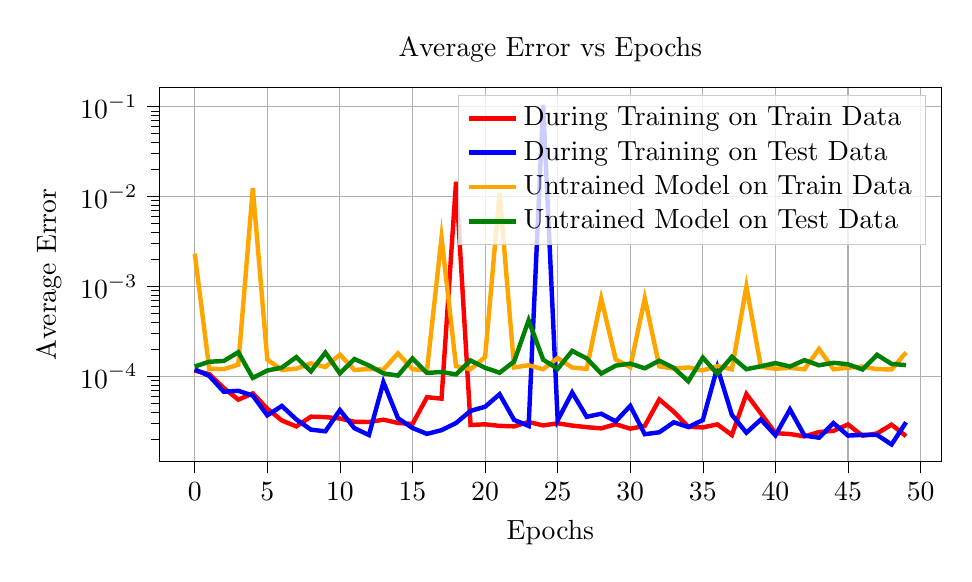
\begin{tikzpicture}

  \definecolor{darkgray176}{RGB}{176,176,176}
  \definecolor{green}{RGB}{0,128,0}
  \definecolor{lightgray204}{RGB}{204,204,204}
  \definecolor{orange}{RGB}{255,165,0}
  
  \begin{axis}[
    width = 0.95\textwidth,
    height = 18em,
  legend cell align={left},
  legend style={
    fill opacity=0.8,
    draw opacity=1,
    text opacity=1,
    % at={(0.91,0.5)},
    % anchor=east,
    draw=lightgray204
  },
  % log basis y={10},
  tick align=outside,
  tick pos=left,
  title={Average Error vs Epochs},
  x grid style={darkgray176},
  xlabel={Epochs},
  xmajorgrids,
  xmin=-2.45, xmax=51.45,
  xtick style={color=black},
  y grid style={darkgray176},
  ylabel={Average Error},
  ymajorgrids,
  ymin=1.13394664622616e-05, ymax=0.161938808815307,
ymode=log,
ytick style={color=black},
ytick={1e-06,1e-05,0.0001,0.001,0.01,0.1,1,10},
yticklabels={
  \(\displaystyle {10^{-6}}\),
  \(\displaystyle {10^{-5}}\),
  \(\displaystyle {10^{-4}}\),
  \(\displaystyle {10^{-3}}\),
  \(\displaystyle {10^{-2}}\),
  \(\displaystyle {10^{-1}}\),
  \(\displaystyle {10^{0}}\),
  \(\displaystyle {10^{1}}\)
}
]
\addplot [ultra thick, red]
table {%
0 0.000115964649012312
1 0.000106160565337632
2 7.4514202424325e-05
3 5.52686251467094e-05
4 6.47887063678354e-05
5 4.38010902144015e-05
6 3.23934727930464e-05
7 2.78183033515234e-05
8 3.57124663423747e-05
9 3.53135837940499e-05
10 3.40799015248194e-05
11 3.13175551127642e-05
12 3.11450057779439e-05
13 3.30704897351097e-05
14 3.04046770907007e-05
15 2.96264006465208e-05
16 5.87791255384218e-05
17 5.6647138990229e-05
18 0.0146533735096455
19 2.88673472823575e-05
20 2.93554567178944e-05
21 2.82165401586099e-05
22 2.787177436403e-05
23 3.11427174892742e-05
24 2.85501137113897e-05
25 3.01203654089477e-05
26 2.84152793028625e-05
27 2.73057776212227e-05
28 2.64660557149909e-05
29 2.9429202186293e-05
30 2.62424036918674e-05
31 2.8169297365821e-05
32 5.54843718418851e-05
33 4.05666069127619e-05
34 2.75754628091818e-05
35 2.71147255261894e-05
36 2.93161992885871e-05
37 2.23202241613762e-05
38 6.3687919464428e-05
39 3.87190993933473e-05
40 2.34123890550109e-05
41 2.28933477046667e-05
42 2.15512700378895e-05
43 2.40790013776859e-05
44 2.48580217885319e-05
45 2.92275672109099e-05
46 2.18897512240801e-05
47 2.32488600886427e-05
48 2.91028009087313e-05
49 2.16724984056782e-05
};
\addlegendentry{During Training on Train Data}
\addplot [ultra thick, blue]
table {%
0 0.000119965603516903
1 0.000101332203485072
2 6.76928320899606e-05
3 6.92283501848578e-05
4 6.13137017353438e-05
5 3.69310146197677e-05
6 4.69658516522031e-05
7 3.3255073503824e-05
8 2.56295552389929e-05
9 2.45451210503234e-05
10 4.22778066422325e-05
11 2.65813923761016e-05
12 2.23145234485855e-05
13 8.61937660374679e-05
14 3.43234569299966e-05
15 2.67034629359841e-05
16 2.29790675803088e-05
17 2.527412470954e-05
18 3.0333951144712e-05
19 4.13999114243779e-05
20 4.60761657450348e-05
21 6.34397874819115e-05
22 3.28440728480928e-05
23 2.81884076684946e-05
24 0.10483306646347
25 3.2550346077187e-05
26 6.62766105961055e-05
27 3.55897900590207e-05
28 3.84878294426017e-05
29 3.16521618515253e-05
30 4.70157174277119e-05
31 2.27859763981542e-05
32 2.39355322264601e-05
33 3.09546412609052e-05
34 2.7367514121579e-05
35 3.2791547710076e-05
36 0.000126061495393515
37 3.74597329937387e-05
38 2.36853138630977e-05
39 3.31944938807283e-05
40 2.21443497139262e-05
41 4.30283471359871e-05
42 2.20024030568311e-05
43 2.08455585379852e-05
44 3.03072501992574e-05
45 2.1999707314535e-05
46 2.23901915887836e-05
47 2.24012856051559e-05
48 1.75164168467745e-05
49 3.0965751648182e-05
};
\addlegendentry{During Training on Test Data}
\addplot [ultra thick, orange]
table {%
0 0.00232795067131519
1 0.000121869074064307
2 0.000120698474347591
3 0.000135069276439026
4 0.0124339954927564
5 0.000153945249621756
6 0.000118231007945724
7 0.000122039848065469
8 0.000140186384669505
9 0.00012726680142805
10 0.000174994856934063
11 0.000118236494017765
12 0.000121040582598653
13 0.000119276381155942
14 0.000180863629793748
15 0.00012022288137814
16 0.000117313240480144
17 0.00351618696004152
18 0.000130253116367385
19 0.00012056008563377
20 0.000164105353178456
21 0.0109988208860159
22 0.000125871316413395
23 0.000133313849801198
24 0.000120252356282435
25 0.000160284704179503
26 0.000125728212879039
27 0.000121358069009148
28 0.000733525725081563
29 0.000154539637151174
30 0.000126869344967417
31 0.000736654968932271
32 0.000129571038996801
33 0.000122085199109279
34 0.000125906270113774
35 0.000116696552140638
36 0.000130216154502705
37 0.000120131124276668
38 0.000999922631308436
39 0.000127725084894337
40 0.000121914374176413
41 0.000124539728858508
42 0.000120200413221028
43 0.000201997492695227
44 0.000120335920655634
45 0.000125129503430799
46 0.000128802537801675
47 0.000120474636787549
48 0.00011976600944763
49 0.00018517866556067
};
\addlegendentry{Untrained Model on Train Data}
\addplot [ultra thick, green]
table {%
0 0.000129062638734467
1 0.000145741840242408
2 0.000148645412991755
3 0.000185903554665856
4 9.62841222644784e-05
5 0.00011643586185528
6 0.000125509759527631
7 0.000164188357302919
8 0.000113728274300229
9 0.000184246688149869
10 0.000108123131212778
11 0.000156331152538769
12 0.000132504908833653
13 0.00010812053369591
14 0.000102231824712362
15 0.000158902883413248
16 0.000109439031803049
17 0.000112151916255243
18 0.000105350838566665
19 0.000150613894220442
20 0.000124783167848364
21 0.000110051209048834
22 0.000146668040542863
23 0.00042110844515264
24 0.000153782195411623
25 0.000121453274914529
26 0.000192303283256479
27 0.000158814698806964
28 0.000107618201582227
29 0.00013192389451433
30 0.000138851260999218
31 0.000123196819913574
32 0.000149802639498375
33 0.000124568658065982
34 8.8295120804105e-05
35 0.000161883814143948
36 0.000107056694105268
37 0.000165244477102533
38 0.000120437529403716
39 0.000129807071061805
40 0.000140801450470462
41 0.000128936153487302
42 0.000151907806866802
43 0.000133040055516176
44 0.000141951051773503
45 0.000136660790303722
46 0.000119454423838761
47 0.000174097032868303
48 0.000137830531457439
49 0.000133577806991525
};
\addlegendentry{Untrained Model on Test Data}
\end{axis}

\end{tikzpicture}
}\\
  \subfloat[Different Scalars$(\tau_k)$, $lr=1.000\times10^{-3}$]{% This file was created with tikzplotlib v0.10.1.
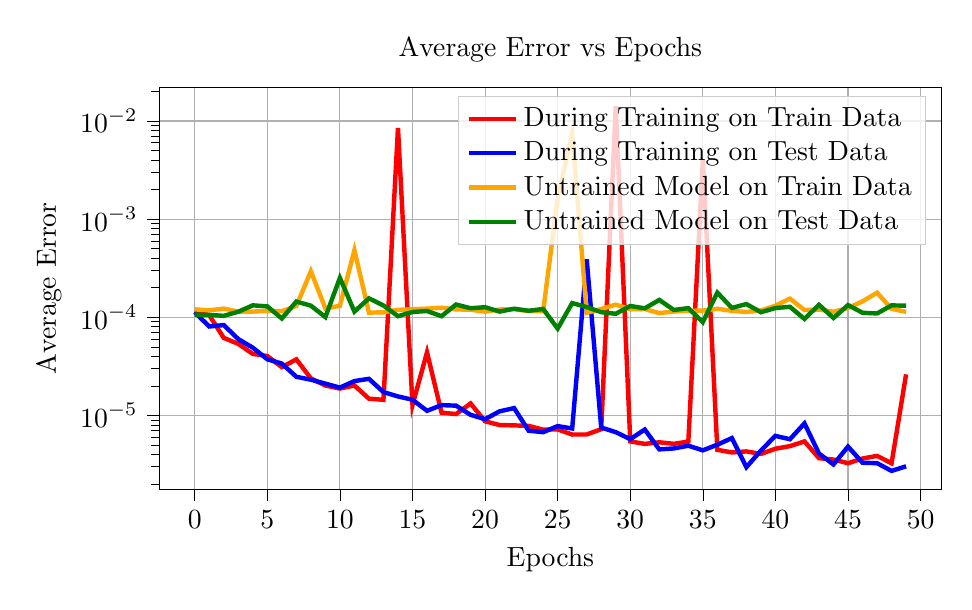
\begin{tikzpicture}

    \definecolor{darkgray176}{RGB}{176,176,176}
    \definecolor{green}{RGB}{0,128,0}
    \definecolor{lightgray204}{RGB}{204,204,204}
    \definecolor{orange}{RGB}{255,165,0}
    
    \begin{axis}[
      width = 0.95\textwidth,
      height = 19em,
    legend cell align={left},
    legend style={
      fill opacity=0.8,
      draw opacity=1,
      text opacity=1,
      % at={(0.91,0.5)},
      % anchor=east,
      draw=lightgray204
    },
    % log basis y={10},
    tick align=outside,
    tick pos=left,
    title={Average Error vs Epochs},
    x grid style={darkgray176},
    xlabel={Epochs},
    xmajorgrids,
    xmin=-2.45, xmax=51.45,
    xtick style={color=black},
    y grid style={darkgray176},
    ylabel={Average Error},
    ymajorgrids,
    ymin=1.77265045649501e-06, ymax=0.0217257085799638,
ymode=log,
ytick style={color=black},
ytick={1e-07,1e-06,1e-05,0.0001,0.001,0.01,0.1,1},
yticklabels={
  \(\displaystyle {10^{-7}}\),
  \(\displaystyle {10^{-6}}\),
  \(\displaystyle {10^{-5}}\),
  \(\displaystyle {10^{-4}}\),
  \(\displaystyle {10^{-3}}\),
  \(\displaystyle {10^{-2}}\),
  \(\displaystyle {10^{-1}}\),
  \(\displaystyle {10^{0}}\)
}
]
\addplot [ultra thick, red]
table {%
0 0.000116249197162688
1 0.000104777733213268
2 6.16174802416936e-05
3 5.35397994099185e-05
4 4.22738339693751e-05
5 4.02698206016794e-05
6 3.1009447411634e-05
7 3.72181639249902e-05
8 2.38204429479083e-05
9 2.01366219698684e-05
10 1.8768372683553e-05
11 2.01797083718702e-05
12 1.48041463035042e-05
13 1.4403810382646e-05
14 0.00846845842897892
15 1.27274661281263e-05
16 4.39258001279086e-05
17 1.06620564110926e-05
18 1.03143329397426e-05
19 1.32283394123078e-05
20 8.70245912665268e-06
21 7.9739720604266e-06
22 7.91216280049412e-06
23 7.81663038651459e-06
24 7.15070973456022e-06
25 7.19865693099564e-06
26 6.38139272268745e-06
27 6.38953406451037e-06
28 7.23988569006906e-06
29 0.01416249666363
30 5.43188207302592e-06
31 5.12640826855204e-06
32 5.32065496372525e-06
33 5.13297209181474e-06
34 5.40986866326421e-06
35 0.00397870503365993
36 4.45748082711361e-06
37 4.19193565903697e-06
38 4.29415240432718e-06
39 4.04746242566034e-06
40 4.57452460977947e-06
41 4.86139288113918e-06
42 5.43156011190149e-06
43 3.66582253263914e-06
44 3.54837652594142e-06
45 3.25559403790976e-06
46 3.63603157893522e-06
47 3.86781039196649e-06
48 3.25598648487357e-06
49 2.61864806816448e-05
};
\addlegendentry{During Training on Train Data}
\addplot [ultra thick, blue]
table {%
0 0.000112263674964197
1 8.04891242296435e-05
2 8.31869256217033e-05
3 5.98654623900075e-05
4 4.89498270326294e-05
5 3.72918257198762e-05
6 3.3739663194865e-05
7 2.4729093638598e-05
8 2.31083031394519e-05
9 2.10517519008135e-05
10 1.91858325706562e-05
11 2.23716870095814e-05
12 2.35791285376763e-05
13 1.72630680026487e-05
14 1.55992747750133e-05
15 1.44481573443045e-05
16 1.11354383989237e-05
17 1.27217863337137e-05
18 1.25628239402431e-05
19 1.01310497484519e-05
20 9.15393957257038e-06
21 1.09975608211244e-05
22 1.18624620881747e-05
23 6.98091344020213e-06
24 6.74611374051892e-06
25 7.77813875174616e-06
26 7.35434741727659e-06
27 0.000388607470085844
28 7.51973493606783e-06
29 6.748153737135e-06
30 5.72535964238341e-06
31 7.17473221811815e-06
32 4.50263542006724e-06
33 4.60407500213478e-06
34 4.90940510644577e-06
35 4.40480425822898e-06
36 5.02696912008105e-06
37 5.87127215112559e-06
38 2.96681491818163e-06
39 4.38676352132461e-06
40 6.17989599049906e-06
41 5.71354394196533e-06
42 8.28803877084283e-06
43 4.08831328968517e-06
44 3.16428372570954e-06
45 4.80631888422067e-06
46 3.29530416820489e-06
47 3.25893643093877e-06
48 2.71930070994131e-06
49 3.02756961900741e-06
};
\addlegendentry{During Training on Test Data}
\addplot [ultra thick, orange]
table {%
0 0.000120269258331973
1 0.000117629810119979
2 0.000122440571431071
3 0.000114334048703313
4 0.000114169095468242
5 0.000116113071271684
6 0.000115084993012715
7 0.000130586326122284
8 0.000293938588583842
9 0.000122917335829698
10 0.00013070237764623
11 0.000482346513308585
12 0.000111455316073261
13 0.000112260117020924
14 0.000119041971629485
15 0.000120722070278134
16 0.00012233828601893
17 0.000125074948300608
18 0.000120170683658216
19 0.00011924283899134
20 0.000114032402052544
21 0.000119969517982099
22 0.000120646553114057
23 0.000115742535854224
24 0.000115109338366892
25 0.00161717541050166
26 0.00751296384260058
27 0.000110919230792206
28 0.00012136172153987
29 0.000134457382955588
30 0.000120748292829376
31 0.000121317578305025
32 0.000110163149656728
33 0.00011455421190476
34 0.000116186180093791
35 0.000116979601443745
36 0.000121848745038733
37 0.000116133829578757
38 0.000113216083263978
39 0.000117256036901381
40 0.000131090360810049
41 0.000154755791299976
42 0.000118435942567885
43 0.000119846772577148
44 0.000113804286229424
45 0.000124071579193696
46 0.000145310332300141
47 0.000177828187588602
48 0.000121933335321955
49 0.000113341317046434
};
\addlegendentry{Untrained Model on Train Data}
\addplot [ultra thick, green]
table {%
0 0.000106313964352012
1 0.000105647886812221
2 0.000103366750408895
3 0.000113759066152852
4 0.000132218236103654
5 0.000128917745314538
6 9.70740729826503e-05
7 0.000144520294270478
8 0.00013117839989718
9 0.000100422148534562
10 0.000251530116656795
11 0.000114149901492056
12 0.000155831527081318
13 0.000131669556139968
14 0.000102509882708546
15 0.000113139096356463
16 0.000115782873763237
17 0.000102498932392336
18 0.000134782283566892
19 0.000123556092148647
20 0.000126511658891104
21 0.000114194604975637
22 0.000122136902064085
23 0.000116400944534689
24 0.000121366094390396
25 7.6622687629424e-05
26 0.000139483527163975
27 0.000126818413264118
28 0.000112633853859734
29 0.000108447231468745
30 0.000130197833641432
31 0.000123179153888486
32 0.000150192689034157
33 0.000118637071864214
34 0.000123824764159508
35 8.92329844646156e-05
36 0.000178371163201518
37 0.000124380996567197
38 0.000136194779770449
39 0.000112504290882498
40 0.000124128026072867
41 0.000127703809994273
42 9.60812903940678e-05
43 0.000133860929054208
44 9.82828350970522e-05
45 0.000132986911921762
46 0.00011109155457234
47 0.000109223496110644
48 0.000132101107737981
49 0.000131110078655183
};
\addlegendentry{Untrained Model on Test Data}
\end{axis}

\end{tikzpicture}
}\\
  \subfloat[Single Matrix$(\boldsymbol{M})$, $lr=1.000\times10^{-3}$]{% This file was created with tikzplotlib v0.10.1.
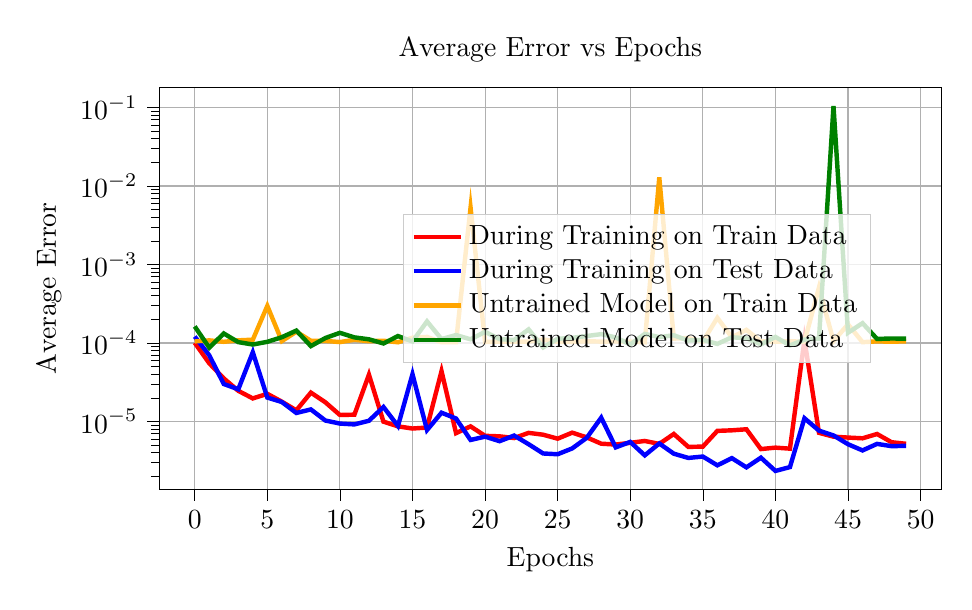
\begin{tikzpicture}

  \definecolor{darkgray176}{RGB}{176,176,176}
  \definecolor{green}{RGB}{0,128,0}
  \definecolor{lightgray204}{RGB}{204,204,204}
  \definecolor{orange}{RGB}{255,165,0}
  
  \begin{axis}[
    width = 0.95\textwidth,
    height = 19em,
  legend cell align={left},
  legend style={
    fill opacity=0.8,
    draw opacity=1,
    text opacity=1,
    at={(0.91,0.5)},
    anchor=east,
    draw=lightgray204
  },
  % log basis y={10},
  tick align=outside,
  tick pos=left,
  title={Average Error vs Epochs},
  x grid style={darkgray176},
  xlabel={Epochs},
  xmajorgrids,
  xmin=-2.45, xmax=51.45,
  xtick style={color=black},
  y grid style={darkgray176},
  ylabel={Average Error},
  ymajorgrids,
  ymin=1.37307878496665e-06, ymax=0.177846155019824,
ymode=log,
ytick style={color=black},
ytick={1e-07,1e-06,1e-05,0.0001,0.001,0.01,0.1,1,10},
yticklabels={
  \(\displaystyle {10^{-7}}\),
  \(\displaystyle {10^{-6}}\),
  \(\displaystyle {10^{-5}}\),
  \(\displaystyle {10^{-4}}\),
  \(\displaystyle {10^{-3}}\),
  \(\displaystyle {10^{-2}}\),
  \(\displaystyle {10^{-1}}\),
  \(\displaystyle {10^{0}}\),
  \(\displaystyle {10^{1}}\)
}
]
\addplot [ultra thick, red]
table {%
0 0.000100550205388572
1 5.51480588910636e-05
2 3.5376513551455e-05
3 2.45903993345564e-05
4 1.96682776731905e-05
5 2.25053372560069e-05
6 1.78705213329522e-05
7 1.38656941999216e-05
8 2.33041700994363e-05
9 1.75389577634633e-05
10 1.20915501611307e-05
11 1.22163710329914e-05
12 3.94555172533728e-05
13 9.94717083813157e-06
14 8.66588470671559e-06
15 8.12911912362324e-06
16 8.36843628349015e-06
17 4.37713715655264e-05
18 7.10201402398525e-06
19 8.66146274347557e-06
20 6.56404654364451e-06
21 6.46528542347369e-06
22 6.1509813349403e-06
23 7.15849364496535e-06
24 6.78525930197793e-06
25 6.03655644226819e-06
26 7.20456819180981e-06
27 6.27475947112544e-06
28 5.21144374943106e-06
29 5.08226366946474e-06
30 5.34771334059769e-06
31 5.64463289265404e-06
32 5.18060278409394e-06
33 6.93121137373964e-06
34 4.74545822726213e-06
35 4.78483070764923e-06
36 7.58898931962904e-06
37 7.7153699749033e-06
38 7.95855885371566e-06
39 4.45058958575828e-06
40 4.64240429209895e-06
41 4.50455945610884e-06
42 0.000109414861071855
43 7.1724243753124e-06
44 6.40393318462884e-06
45 6.23621372142225e-06
46 6.10479764873162e-06
47 6.92588446327136e-06
48 5.43964370081085e-06
49 5.19705054102815e-06
};
\addlegendentry{During Training on Train Data}
\addplot [ultra thick, blue]
table {%
0 0.000120791839435697
1 6.97270734235644e-05
2 3.00260344374692e-05
3 2.56979237747146e-05
4 7.61366973165423e-05
5 2.01856510102516e-05
6 1.7695394490147e-05
7 1.28419051179662e-05
8 1.4239049050957e-05
9 1.02809890449862e-05
10 9.40511290536961e-06
11 9.17238776310114e-06
12 1.02190724646789e-05
13 1.52930533658946e-05
14 8.76629474078072e-06
15 4.00103817810304e-05
16 7.77208060753765e-06
17 1.29295967781218e-05
18 1.09010425148881e-05
19 5.81508083996596e-06
20 6.4081177697517e-06
21 5.60884700462339e-06
22 6.61514650346362e-06
23 5.13239729116322e-06
24 3.91138337363373e-06
25 3.8252628655755e-06
26 4.53538950750954e-06
27 6.18455396761419e-06
28 1.11798572106636e-05
29 4.6780855882389e-06
30 5.49044807485188e-06
31 3.70292764273472e-06
32 5.24500364917913e-06
33 3.88661010219948e-06
34 3.4318647976761e-06
35 3.57546377927065e-06
36 2.76254536402121e-06
37 3.40951532962208e-06
38 2.6036304916488e-06
39 3.45822490999126e-06
40 2.34463345805125e-06
41 2.62418188867741e-06
42 1.0984908840328e-05
43 7.6518654168467e-06
44 6.64355184198939e-06
45 5.13065879204078e-06
46 4.27781515099923e-06
47 5.18121805725968e-06
48 4.84617430629442e-06
49 4.89258400193648e-06
};
\addlegendentry{During Training on Test Data}
\addplot [ultra thick, orange]
table {%
0 0.00010484314407222
1 0.000107949126686435
2 0.000103496546216775
3 0.00010804993507918
4 0.000110162152850535
5 0.000296750164125115
6 0.00010558851499809
7 0.000139229741762392
8 0.000106780855276156
9 0.000106322971987538
10 0.000102692516520619
11 0.000109833126771264
12 0.00010538525384618
13 0.000106810737634078
14 0.000102086036349647
15 0.000116774193884339
16 0.000119435600936413
17 0.000102182850241661
18 0.000102641686680727
19 0.00530683295801282
20 0.000103274374851026
21 0.000103942598798312
22 0.000103939244581852
23 0.000104276216006838
24 0.000110928223875817
25 0.000103578386188019
26 0.000103336431493517
27 0.000105195016658399
28 0.000104166712844744
29 0.000104556929727551
30 0.000103958751424216
31 0.00010203668352915
32 0.0128590352833271
33 0.000113665089884307
34 0.000115690469101537
35 0.000104450569779146
36 0.000209172590984963
37 0.000118048126751091
38 0.0001468143746024
39 0.000105119623185601
40 0.000103922306152526
41 0.000104989230749197
42 0.000103922313428484
43 0.000509256205987185
44 0.000105649472970981
45 0.000173034990439191
46 0.000102450037957169
47 0.00010490239947103
48 0.000103624282928649
49 0.000105106271803379
};
\addlegendentry{Untrained Model on Train Data}
\addplot [ultra thick, green]
table {%
0 0.000162609125254676
1 8.71792071848176e-05
2 0.000132129905978218
3 0.000102534242614638
4 9.55780051299371e-05
5 0.000103471626061946
6 0.00011843147512991
7 0.000143871642649174
8 9.12305331439711e-05
9 0.000115696624561679
10 0.000134690388222225
11 0.000117837000289001
12 0.00011143229494337
13 9.86462255241349e-05
14 0.000122453842777759
15 0.000104537131846882
16 0.000188419173355214
17 0.000112128611363005
18 0.000126249200548045
19 0.000111318797280546
20 0.000138589079142548
21 0.000112062720290851
22 0.000109058710222598
23 0.000148940816870891
24 8.78246864886023e-05
25 0.00011311150592519
26 0.000116243281809147
27 0.00012264410906937
28 0.000129606036352925
29 0.000117648742161691
30 9.57143638515845e-05
31 0.000130468906718306
32 0.000118919684609864
33 0.0001254016533494
34 0.000107390391349327
35 0.00010970434959745
36 9.73197384155355e-05
37 0.000118234478577506
38 0.000114819522423204
39 9.58838500082493e-05
40 0.000119389638712164
41 9.30892638280056e-05
42 0.000110404413135257
43 0.000113703594252001
44 0.104151368141174
45 0.000135112306452356
46 0.000178929112735204
47 0.000112616180558689
48 0.000114114074676763
49 0.000113444977614563
};
\addlegendentry{Untrained Model on Test Data}
\end{axis}

\end{tikzpicture}
}\\  
  \caption{Training the \ac{UWF} Algorithm in different Scenarios Without Optuna\cite{Akiba2019}}
  \label{fig:uwf_training_01_02_03}
  \end{figure}
%   \clearpage % End the page
}
\afterpage{%
%   \clearpage % Start a new page
\begin{figure}[!htbp]
  \subfloat[Single Semi-Positive Definite Matrix$(\boldsymbol{S})$, $lr=1.000\times10^{-3}$]{% This file was created with tikzplotlib v0.10.1.
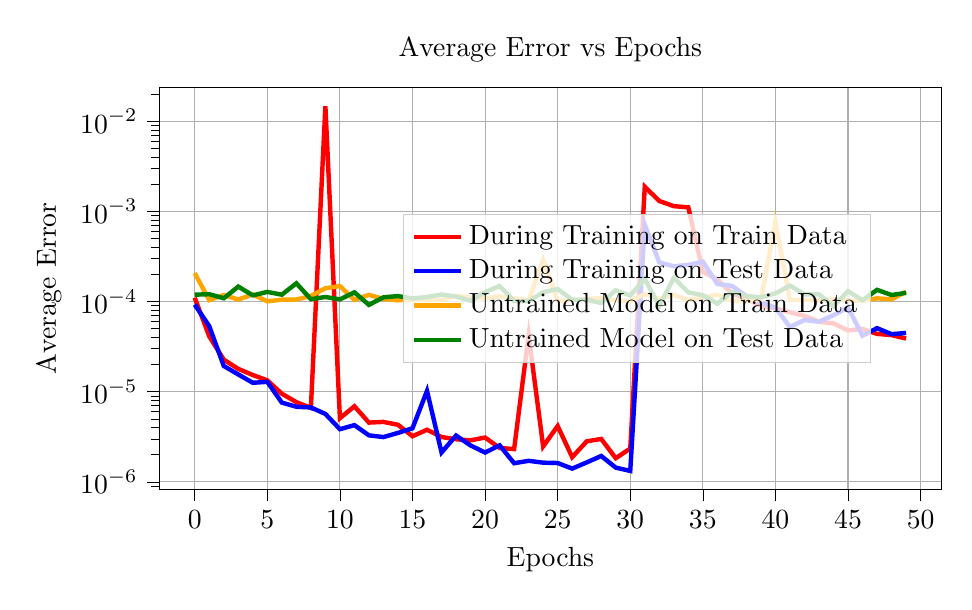
\begin{tikzpicture}

  \definecolor{darkgray176}{RGB}{176,176,176}
  \definecolor{green}{RGB}{0,128,0}
  \definecolor{lightgray204}{RGB}{204,204,204}
  \definecolor{orange}{RGB}{255,165,0}
  
  \begin{axis}[
    width = 0.95\textwidth,
    height = 19em,
  legend cell align={left},
  legend style={
    fill opacity=0.8,
    draw opacity=1,
    text opacity=1,
    at={(0.91,0.5)},
    anchor=east,
    draw=lightgray204
  },
  % log basis y={10},
  tick align=outside,
  tick pos=left,
  title={Average Error vs Epochs},
  x grid style={darkgray176},
  xlabel={Epochs},
  xmajorgrids,
  xmin=-2.45, xmax=51.45,
  xtick style={color=black},
  y grid style={darkgray176},
  ylabel={Average Error},
  ymajorgrids,
  ymin=8.30356451495163e-07, ymax=0.0234483376377019,
  ymode=log,
  ytick style={color=black},
  ytick={1e-08,1e-07,1e-06,1e-05,0.0001,0.001,0.01,0.1,1},
  yticklabels={
    \(\displaystyle {10^{-8}}\),
    \(\displaystyle {10^{-7}}\),
    \(\displaystyle {10^{-6}}\),
    \(\displaystyle {10^{-5}}\),
    \(\displaystyle {10^{-4}}\),
    \(\displaystyle {10^{-3}}\),
    \(\displaystyle {10^{-2}}\),
    \(\displaystyle {10^{-1}}\),
    \(\displaystyle {10^{0}}\)
  }
  ]
  \addplot [ultra thick, red]
  table {%
  0 0.00011017140786862
  1 4.11059882026166e-05
  2 2.26791598834097e-05
  3 1.79246799234534e-05
  4 1.5320852980949e-05
  5 1.33630046548205e-05
  6 9.5052946562646e-06
  7 7.66472021496156e-06
  8 6.61656895317719e-06
  9 0.0147163737565279
  10 5.08682569488883e-06
  11 6.89014314048109e-06
  12 4.54574956165743e-06
  13 4.62558455183171e-06
  14 4.29807005275507e-06
  15 3.20831509270647e-06
  16 3.78796448785579e-06
  17 3.14419253300002e-06
  18 2.96950793199358e-06
  19 2.8898784876219e-06
  20 3.10484847432235e-06
  21 2.37921130974428e-06
  22 2.31052422350331e-06
  23 4.23871242674068e-05
  24 2.47495540861564e-06
  25 4.16208604292478e-06
  26 1.87935143003415e-06
  27 2.81569600701914e-06
  28 2.99561907013413e-06
  29 1.83097131412069e-06
  30 2.34298590839899e-06
  31 0.00187448516953737
  32 0.00130452052690089
  33 0.00114362325984985
  34 0.00110848690383136
  35 0.000213812745641917
  36 0.000175953828147613
  37 0.000123330348287709
  38 0.000108028660179116
  39 8.94952609087341e-05
  40 8.3952174463775e-05
  41 7.61759874876589e-05
  42 6.94747795932926e-05
  43 5.97251892031636e-05
  44 5.72363132960163e-05
  45 4.79114059999119e-05
  46 4.97014989377931e-05
  47 4.38004644820467e-05
  48 4.24669815402012e-05
  49 3.88910702895373e-05
  };
  \addlegendentry{During Training on Train Data}
  \addplot [ultra thick, blue]
  table {%
  0 9.25490385270678e-05
  1 5.33596867171582e-05
  2 1.93084251804976e-05
  3 1.55448160512606e-05
  4 1.25676324387314e-05
  5 1.28699921333464e-05
  6 7.57245152271935e-06
  7 6.81047959005809e-06
  8 6.69457676849561e-06
  9 5.67144479646231e-06
  10 3.838911652565e-06
  11 4.25930056735524e-06
  12 3.28157580042898e-06
  13 3.14029966830276e-06
  14 3.49249467035406e-06
  15 3.93286927646841e-06
  16 1.021505886456e-05
  17 2.12089162232587e-06
  18 3.26139775097545e-06
  19 2.53603025157645e-06
  20 2.11525298254855e-06
  21 2.54228211815644e-06
  22 1.61134596510237e-06
  23 1.71185638464522e-06
  24 1.63372749284463e-06
  25 1.61897480666084e-06
  26 1.4033945490155e-06
  27 1.64422237958206e-06
  28 1.93664232028823e-06
  29 1.43909312555479e-06
  30 1.3230486501925e-06
  31 0.000710018270183355
  32 0.000271758821327239
  33 0.000246446783421561
  34 0.000255026272498071
  35 0.000276810955256224
  36 0.000156756999786012
  37 0.000149476327351294
  38 0.00011513374192873
  39 9.80292679741979e-05
  40 8.57639533933252e-05
  41 5.22035370522644e-05
  42 6.24703752691858e-05
  43 5.97249963902868e-05
  44 7.06285718479194e-05
  45 8.5684958321508e-05
  46 4.18876697949599e-05
  47 5.06847063661553e-05
  48 4.34827052231412e-05
  49 4.48781538580079e-05
  };
  \addlegendentry{During Training on Test Data}
  \addplot [ultra thick, orange]
  table {%
  0 0.000206905984668992
  1 0.000103879472590052
  2 0.000118318079330493
  3 0.000105264494777657
  4 0.000119957672723103
  5 0.000100582859886345
  6 0.000104946513602044
  7 0.00010529812425375
  8 0.000115304595965426
  9 0.00014042342081666
  10 0.000148564169649035
  11 0.000104292754258495
  12 0.000118672374810558
  13 0.000106923791463487
  14 0.000103263271739706
  15 0.000104954779089894
  16 0.000105238294054288
  17 0.000103833881439641
  18 0.000116424649604596
  19 0.00011088097380707
  20 0.000108337342680898
  21 0.000114240865514148
  22 0.000109240827441681
  23 0.000102296020486392
  24 0.000289732008241117
  25 0.000101823032309767
  26 0.000103681690234225
  27 0.000106592997326516
  28 0.000109664819319732
  29 0.000102982463431545
  30 0.000100728902907576
  31 0.000121338045573793
  32 0.000106943414721172
  33 0.00011857563367812
  34 0.000104435559478588
  35 0.000110423032310791
  36 0.000119195072329603
  37 0.000101302670373116
  38 0.000102362369943876
  39 0.000105079387139995
  40 0.000755981716793031
  41 0.000104519625892863
  42 0.000104554841527715
  43 0.00010283276787959
  44 0.000106273328128736
  45 0.000103005295386538
  46 0.000101797762908973
  47 0.00010864141950151
  48 0.000105727842310444
  49 0.000129021689645015
  };
  \addlegendentry{Untrained Model on Train Data}
  \addplot [ultra thick, green]
  table {%
  0 0.000119204923976213
  1 0.000120657336083241
  2 0.000108705302409362
  3 0.000146574966493063
  4 0.000117096795293037
  5 0.000127962775877677
  6 0.000119190335681196
  7 0.000159544200869277
  8 0.000106249608506914
  9 0.00011236439604545
  10 0.000105749604699668
  11 0.000126424361951649
  12 9.19119192985818e-05
  13 0.000111535264295526
  14 0.000114964313979726
  15 0.000108208543679211
  16 0.000112283334601671
  17 0.000119772463222034
  18 0.000113725291157607
  19 0.000101854733657092
  20 0.000127379506011494
  21 0.000148780411109328
  22 0.000101492019894067
  23 0.000100914112408645
  24 0.000126960148918442
  25 0.000137646900839172
  26 0.000104842918517534
  27 0.000104761616967153
  28 9.63836064329371e-05
  29 0.00013338343705982
  30 0.000116854433144908
  31 0.000178153422893956
  32 8.89116417965852e-05
  33 0.000183252937858924
  34 0.000126386919873767
  35 0.000117637937364634
  36 9.48547967709601e-05
  37 0.000127650404465385
  38 0.000115260736492928
  39 0.000111453024146613
  40 0.000123388235806488
  41 0.000150240593939088
  42 0.000120371230877936
  43 0.00012029549543513
  44 8.89928996912204e-05
  45 0.000130154177895747
  46 0.000103636462881695
  47 0.000134864647407085
  48 0.000118217023555189
  49 0.000124695201520808
  };
  \addlegendentry{Untrained Model on Test Data}
  \end{axis}
  
  \end{tikzpicture}
  }\\
  \subfloat[Different Scalars Plus a Single Matrix$(\tau_k\boldsymbol{M})$, $lr=1.000\times10^{-3}$]{% This file was created with tikzplotlib v0.10.1.
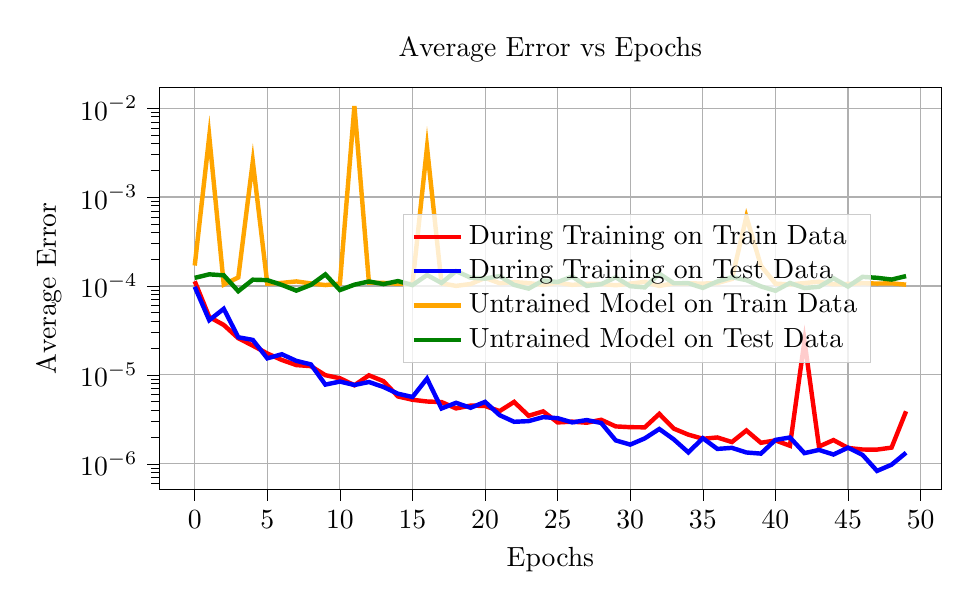
\begin{tikzpicture}

  \definecolor{darkgray176}{RGB}{176,176,176}
  \definecolor{green}{RGB}{0,128,0}
  \definecolor{lightgray204}{RGB}{204,204,204}
  \definecolor{orange}{RGB}{255,165,0}
  
  \begin{axis}[
    width = 0.95\textwidth,
    height = 19em,
  legend cell align={left},
  legend style={
    fill opacity=0.8,
    draw opacity=1,
    text opacity=1,
    at={(0.91,0.5)},
    anchor=east,
    draw=lightgray204
  },
  % log basis y={10},
  tick align=outside,
  tick pos=left,
  title={Average Error vs Epochs},
  x grid style={darkgray176},
  xlabel={Epochs},
  xmajorgrids,
  xmin=-2.45, xmax=51.45,
  xtick style={color=black},
  y grid style={darkgray176},
  ylabel={Average Error},
  ymajorgrids,
  ymin=5.19130698649686e-07, ymax=0.0168909804103019,
ymode=log,
ytick style={color=black},
ytick={1e-08,1e-07,1e-06,1e-05,0.0001,0.001,0.01,0.1,1},
yticklabels={
  \(\displaystyle {10^{-8}}\),
  \(\displaystyle {10^{-7}}\),
  \(\displaystyle {10^{-6}}\),
  \(\displaystyle {10^{-5}}\),
  \(\displaystyle {10^{-4}}\),
  \(\displaystyle {10^{-3}}\),
  \(\displaystyle {10^{-2}}\),
  \(\displaystyle {10^{-1}}\),
  \(\displaystyle {10^{0}}\)
}
]
\addplot [ultra thick, red]
table {%
0 0.000112962785351556
1 4.48540376964957e-05
2 3.64356747013517e-05
3 2.58560248767026e-05
4 2.13579842238687e-05
5 1.74112774402602e-05
6 1.4716902114742e-05
7 1.29015252241516e-05
8 1.25480291899294e-05
9 9.9248736660229e-06
10 9.17880970519036e-06
11 7.65304866945371e-06
12 9.89140698948177e-06
13 8.50470587465679e-06
14 5.72539238419267e-06
15 5.25426003150642e-06
16 5.02280590808368e-06
17 4.95167842018418e-06
18 4.19963316744543e-06
19 4.51622054242762e-06
20 4.47754109700327e-06
21 3.91919320463785e-06
22 4.96741358801955e-06
23 3.47205605066847e-06
24 3.88669877793291e-06
25 2.92186609840428e-06
26 2.98198824566498e-06
27 2.90055436380499e-06
28 3.12721545014938e-06
29 2.63544507106417e-06
30 2.58395039054449e-06
31 2.57365741163085e-06
32 3.64444349543191e-06
33 2.48862534135696e-06
34 2.12954569178692e-06
35 1.91410390470992e-06
36 1.97989515982044e-06
37 1.75854495410022e-06
38 2.37311110140581e-06
39 1.72470777215494e-06
40 1.83481017757003e-06
41 1.5974778762029e-06
42 2.41492052737158e-05
43 1.56557496211462e-06
44 1.85024020993296e-06
45 1.50920891428541e-06
46 1.44889315834007e-06
47 1.44598004681029e-06
48 1.52251061535935e-06
49 3.89733122574398e-06
};
\addlegendentry{During Training on Train Data}
\addplot [ultra thick, blue]
table {%
0 9.79704927885905e-05
1 4.12220251746476e-05
2 5.53868012502789e-05
3 2.65078506345162e-05
4 2.47435182245681e-05
5 1.53581186168594e-05
6 1.70738458109554e-05
7 1.43801589729264e-05
8 1.31255337691982e-05
9 7.78157573222416e-06
10 8.41329165268689e-06
11 7.70366295910208e-06
12 8.32178193377331e-06
13 7.31489717509248e-06
14 6.14505415796884e-06
15 5.64179208595306e-06
16 9.09058144316077e-06
17 4.19361049353029e-06
18 4.85428381580277e-06
19 4.2705137275334e-06
20 4.97809787702863e-06
21 3.52773895428982e-06
22 2.96986331704829e-06
23 3.0228309242375e-06
24 3.34979563376692e-06
25 3.26234339809162e-06
26 2.9221325803519e-06
27 3.10721816276782e-06
28 2.88122487290821e-06
29 1.83466761427553e-06
30 1.64603432040167e-06
31 1.93400114767428e-06
32 2.46550166593806e-06
33 1.88306512427516e-06
34 1.34632125536882e-06
35 1.94003655451525e-06
36 1.47169430420035e-06
37 1.51246365476254e-06
38 1.34194874590321e-06
39 1.30329044623068e-06
40 1.85762326054828e-06
41 1.98000816453714e-06
42 1.31961667193536e-06
43 1.43369834404439e-06
44 1.27295731999766e-06
45 1.5204713008643e-06
46 1.26114775866881e-06
47 8.32501086733828e-07
48 9.78654384198308e-07
49 1.33386754441744e-06
};
\addlegendentry{During Training on Test Data}
\addplot [ultra thick, orange]
table {%
0 0.000169708990142681
1 0.00482502207159996
2 0.000103700578620192
3 0.000124842918012291
4 0.00251293904148042
5 0.00010616429062793
6 0.000108305182948243
7 0.000112550253106747
8 0.000106743587821256
9 0.000102433339634445
10 0.000106333405710757
11 0.01053287088871
12 0.000108984153484926
13 0.000108274653030094
14 0.000105925755633507
15 0.000105766543128993
16 0.00362761900760233
17 0.000107082749309484
18 0.000100305762316566
19 0.000105189930764027
20 0.000123338410048746
21 0.000107556705188472
22 0.000110498091089539
23 0.000107814186776523
24 0.000102985890407581
25 0.000109032029286027
26 0.000102884863736108
27 0.000106015671917703
28 0.000105341321614105
29 0.0001019578485284
30 0.000106281739135738
31 0.000111209985334426
32 0.000100089448096696
33 0.000107222200313117
34 0.000107154046418145
35 0.00010641436529113
36 0.00010793480760185
37 0.000119912510854192
38 0.00060050404863432
39 0.000168843835126609
40 0.00010635306534823
41 0.000103974161902443
42 0.000107886335172225
43 0.000111731547804084
44 0.000104657148767728
45 0.000105431492556818
46 0.000107476378616411
47 0.00010649069736246
48 0.000107057414425071
49 0.000103465994470753
};
\addlegendentry{Untrained Model on Train Data}
\addplot [ultra thick, green]
table {%
0 0.000123337187687866
1 0.000135178546770476
2 0.000131734122987837
3 8.73675089678727e-05
4 0.000117682087875437
5 0.000116350223834161
6 0.000102812009572517
7 8.87012283783406e-05
8 0.000102752564998809
9 0.000135041962494142
10 8.99567967280746e-05
11 0.000103442929685116
12 0.000112348607217427
13 0.000105076818726957
14 0.000113511741801631
15 0.000102312733361032
16 0.000132773231598549
17 0.000108219850517344
18 0.000147023776662536
19 0.000124088546726853
20 0.000121150726045016
21 0.000129152715089731
22 0.000102785998024046
23 9.34063136810437e-05
24 0.000115276103315409
25 0.000110873101220932
26 0.000127559003885835
27 0.00010026985546574
28 0.000104789636679925
29 0.000125139951705933
30 9.94918664218858e-05
31 9.63477796176448e-05
32 0.000137592956889421
33 0.000107359723187983
34 0.000107482650491875
35 9.51347683439963e-05
36 0.000112397479824722
37 0.000125626218505204
38 0.000116283241368365
39 9.89372856565751e-05
40 8.84069959283806e-05
41 0.000108127227576915
42 9.48129090829752e-05
43 9.78503885562532e-05
44 0.00012213944864925
45 9.85664883046411e-05
46 0.00012659138883464
47 0.000123616337077692
48 0.000118097093945835
49 0.000129162333905697
};
\addlegendentry{Untrained Model on Test Data}
\end{axis}

\end{tikzpicture}
}\\
  \subfloat[Different Scalars Plus a Single Semi-Positive Definite Matrix$(\tau_k\boldsymbol{S})$, $lr=1.000\times10^{-3}$]{% This file was created with tikzplotlib v0.10.1.
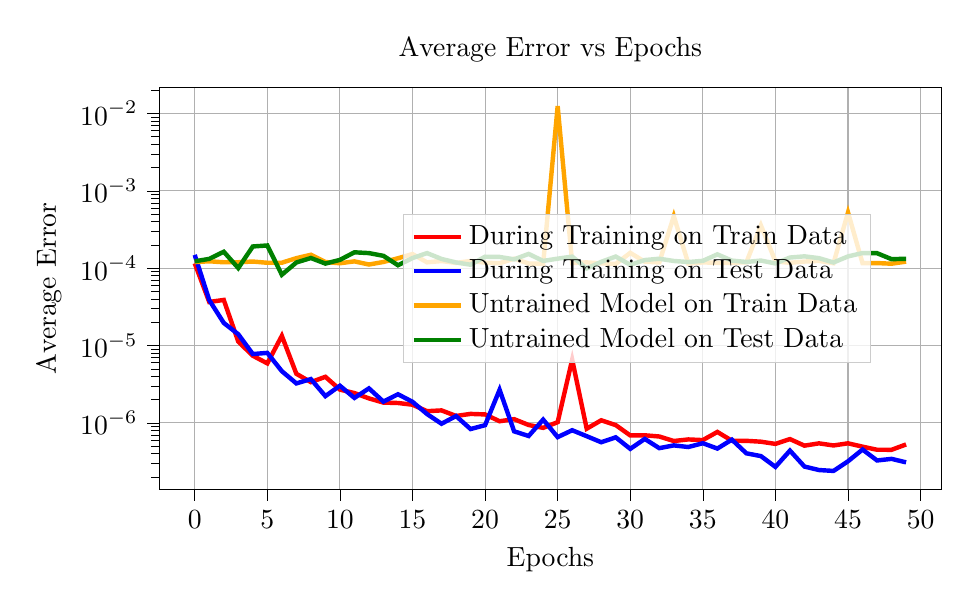
\begin{tikzpicture}

  \definecolor{darkgray176}{RGB}{176,176,176}
  \definecolor{green}{RGB}{0,128,0}
  \definecolor{lightgray204}{RGB}{204,204,204}
  \definecolor{orange}{RGB}{255,165,0}
  
  \begin{axis}[
    width = 0.95\textwidth,
    height = 19em,
  legend cell align={left},
  legend style={
    fill opacity=0.8,
    draw opacity=1,
    text opacity=1,
    at={(0.91,0.5)},
    anchor=east,
    draw=lightgray204
  },
  % log basis y={10},
  tick align=outside,
  tick pos=left,
  title={Average Error vs Epochs},
  x grid style={darkgray176},
  xlabel={Epochs},
  xmajorgrids,
  xmin=-2.45, xmax=51.45,
  xtick style={color=black},
  y grid style={darkgray176},
  ylabel={Average Error},
  ymajorgrids,
  ymin=1.3929386884171e-07, ymax=0.0214137849226391,
ymode=log,
ytick style={color=black},
ytick={1e-08,1e-07,1e-06,1e-05,0.0001,0.001,0.01,0.1,1},
yticklabels={
  \(\displaystyle {10^{-8}}\),
  \(\displaystyle {10^{-7}}\),
  \(\displaystyle {10^{-6}}\),
  \(\displaystyle {10^{-5}}\),
  \(\displaystyle {10^{-4}}\),
  \(\displaystyle {10^{-3}}\),
  \(\displaystyle {10^{-2}}\),
  \(\displaystyle {10^{-1}}\),
  \(\displaystyle {10^{0}}\)
}
]
\addplot [ultra thick, red]
table {%
0 0.000115619572170544
1 3.66140666301362e-05
2 3.88987718906719e-05
3 1.12463349069003e-05
4 7.39141842132085e-06
5 5.88246757615707e-06
6 1.33564672069042e-05
7 4.32045681009186e-06
8 3.36766470354632e-06
9 3.94663265979034e-06
10 2.69568681687815e-06
11 2.43232580032782e-06
12 2.07539164875925e-06
13 1.83115344043472e-06
14 1.81004190835665e-06
15 1.71904935086786e-06
16 1.41902387440496e-06
17 1.45171202348138e-06
18 1.23093161619181e-06
19 1.30822729715874e-06
20 1.28785870856518e-06
21 1.05134529349016e-06
22 1.11863823804015e-06
23 9.40535358040506e-07
24 8.63363482039858e-07
25 1.02263186363416e-06
26 6.57841155771166e-06
27 8.42167764858459e-07
28 1.08156234546186e-06
29 9.38011964990437e-07
30 6.88994134634413e-07
31 6.92170203819842e-07
32 6.67649260321923e-07
33 5.83880023441452e-07
34 6.11951520568255e-07
35 6.00160205976863e-07
36 7.64876006087434e-07
37 5.89186356592108e-07
38 5.87023293974198e-07
39 5.72065005144395e-07
40 5.35504113940988e-07
41 6.18023648257804e-07
42 5.08474954585836e-07
43 5.44603835805901e-07
44 5.11379028012016e-07
45 5.45023794984445e-07
46 4.93479035412747e-07
47 4.499693204707e-07
48 4.4950027699997e-07
49 5.27288420926197e-07
};
\addlegendentry{During Training on Train Data}
\addplot [ultra thick, blue]
table {%
0 0.000148638486280106
1 3.8717822462786e-05
2 1.96167875401443e-05
3 1.40024994834675e-05
4 7.77251534600509e-06
5 8.04341743787518e-06
6 4.66747496830067e-06
7 3.24275606544688e-06
8 3.68673295270128e-06
9 2.22127937377081e-06
10 3.02577313959773e-06
11 2.10539269573928e-06
12 2.79613914244692e-06
13 1.88535034340021e-06
14 2.34871004067827e-06
15 1.87500120318873e-06
16 1.30373712181608e-06
17 9.7612542049319e-07
18 1.22695689697139e-06
19 8.33635738217708e-07
20 9.3538966439155e-07
21 2.68304006567632e-06
22 7.79187587340857e-07
23 6.77797231674049e-07
24 1.10359292193607e-06
25 6.55734368137928e-07
26 8.04333865289664e-07
27 6.73910278692347e-07
28 5.62983984764287e-07
29 6.51476170787646e-07
30 4.62268644696451e-07
31 6.21099786712875e-07
32 4.7201328357005e-07
33 5.12390784024319e-07
34 4.88249042973621e-07
35 5.46861258499121e-07
36 4.66291567136068e-07
37 6.0789801636929e-07
38 4.04685039256947e-07
39 3.72652806390761e-07
40 2.70373163857585e-07
41 4.39054105072501e-07
42 2.73006207862636e-07
43 2.46051911290124e-07
44 2.39714267991076e-07
45 3.1927794452713e-07
46 4.52996403055295e-07
47 3.27289853885304e-07
48 3.43154766824227e-07
49 3.09403873188785e-07
};
\addlegendentry{During Training on Test Data}
\addplot [ultra thick, orange]
table {%
0 0.000119844757136889
1 0.000122850964544341
2 0.000119242758955806
3 0.0001194120341097
4 0.000121909339213744
5 0.000117509182018694
6 0.000117711497296114
7 0.000134808011353016
8 0.000149091443745419
9 0.000120183576655108
10 0.000115898626972921
11 0.000122511555673555
12 0.000111565263068769
13 0.000120325428724755
14 0.000134350819280371
15 0.000152338034240529
16 0.000119035270472523
17 0.00012379974941723
18 0.000117030824185349
19 0.000124024198157713
20 0.000117830757517368
21 0.000115914219350088
22 0.00013274562661536
23 0.00011486293078633
24 0.000114014488644898
25 0.0124431848526001
26 0.000116647170216311
27 0.000118882482638583
28 0.000115469163574744
29 0.000113608708488755
30 0.00015779300883878
31 0.000121383927762508
32 0.000118668504001107
33 0.00047049461863935
34 0.000114619404484984
35 0.00011880121746799
36 0.000117411691462621
37 0.000117397568828892
38 0.000119214426376857
39 0.000357582262950018
40 0.000122612778795883
41 0.000117423463962041
42 0.000121910503366962
43 0.000124323123600334
44 0.000115912305773236
45 0.000524870993103832
46 0.000116180184704717
47 0.000116481249278877
48 0.000114282163849566
49 0.000121571094496176
};
\addlegendentry{Untrained Model on Train Data}
\addplot [ultra thick, green]
table {%
0 0.000122817582450807
1 0.000132000757730566
2 0.000163245917065069
3 0.000100329452834558
4 0.000190929204109125
5 0.000196753637283109
6 8.23061054688878e-05
7 0.000118566029414069
8 0.000135401103761978
9 0.000114686314191204
10 0.000128131257952191
11 0.000160483745275997
12 0.000156743626575917
13 0.000144422388984822
14 0.00010919920168817
15 0.000135145717649721
16 0.000156790585606359
17 0.000131657448946498
18 0.000118700903840363
19 0.000110858003608882
20 0.00014075958461035
21 0.000139842843054794
22 0.000130170141346753
23 0.000152905340655707
24 0.000124135913210921
25 0.000132893052068539
26 0.000141130716656335
27 9.90790795185603e-05
28 0.000120807693747338
29 0.000141456825076602
30 0.000110587214294355
31 0.000127455787151121
32 0.00013254517398309
33 0.00012397175305523
34 0.000120144453831017
35 0.000124459431390278
36 0.000150959225720726
37 0.000125301812659018
38 0.000120412958494853
39 0.000125558653962798
40 0.000115242255560588
41 0.000137347829877399
42 0.000142319564474747
43 0.000134914516820572
44 0.000118584044685122
45 0.000142000455525704
46 0.000157046873937361
47 0.000156261696247384
48 0.000130856220494024
49 0.000132377448608167
};
\addlegendentry{Untrained Model on Test Data}
\end{axis}

\end{tikzpicture}
}\\
  \caption{Training the \ac{UWF} Algorithm in different Scenarios Without Optuna\cite{Akiba2019}}
  \label{fig:uwf_training_04_05_06}
  \end{figure}
%   \clearpage % End the page
}

\afterpage{%
%   \clearpage % Start a new page
\begin{figure}[!htbp]
  \subfloat[Different Matrices$(\boldsymbol{M}_k)$, $lr=1.000\times10^{-3}$]{% This file was created with tikzplotlib v0.10.1.
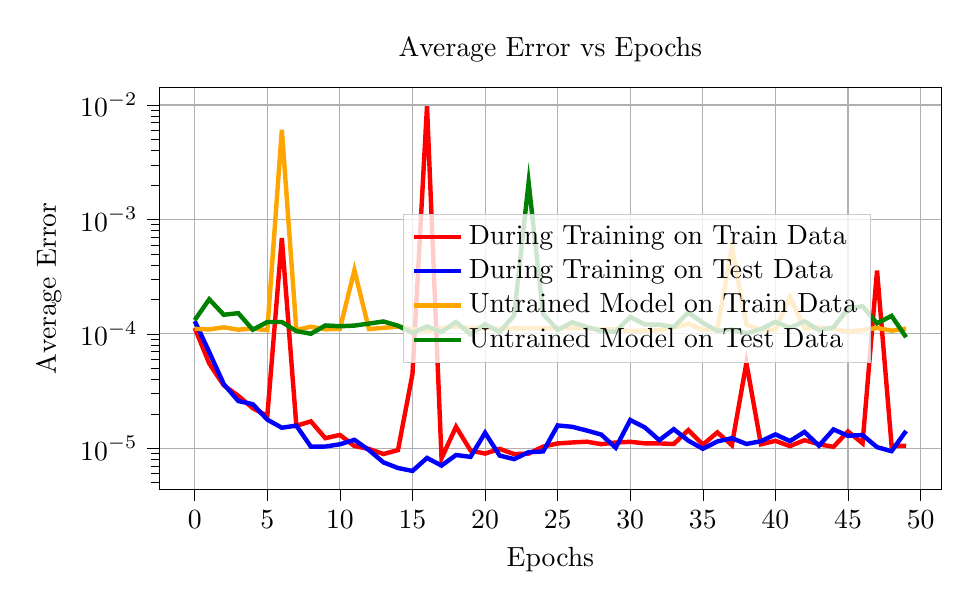
\begin{tikzpicture}

  \definecolor{darkgray176}{RGB}{176,176,176}
  \definecolor{green}{RGB}{0,128,0}
  \definecolor{lightgray204}{RGB}{204,204,204}
  \definecolor{orange}{RGB}{255,165,0}
  
  \begin{axis}[
    width = 0.95\textwidth,
    height = 19em,
  legend cell align={left},
  legend style={
    fill opacity=0.8,
    draw opacity=1,
    text opacity=1,
    at={(0.91,0.5)},
    anchor=east,
    draw=lightgray204
  },
  % log basis y={10},
  tick align=outside,
  tick pos=left,
  title={Average Error vs Epochs},
  x grid style={darkgray176},
  xlabel={Epochs},
  xmajorgrids,
  xmin=-2.45, xmax=51.45,
  xtick style={color=black},
  y grid style={darkgray176},
  ylabel={Average Error},
  ymajorgrids,
  ymin=4.39300939358295e-06, ymax=0.0141089359119069,
ymode=log,
ytick style={color=black},
ytick={1e-07,1e-06,1e-05,0.0001,0.001,0.01,0.1,1},
yticklabels={
  \(\displaystyle {10^{-7}}\),
  \(\displaystyle {10^{-6}}\),
  \(\displaystyle {10^{-5}}\),
  \(\displaystyle {10^{-4}}\),
  \(\displaystyle {10^{-3}}\),
  \(\displaystyle {10^{-2}}\),
  \(\displaystyle {10^{-1}}\),
  \(\displaystyle {10^{0}}\)
}
]
\addplot [ultra thick, red]
table {%
0 0.000112517256638967
1 5.5064581829356e-05
2 3.55100528395269e-05
3 2.87373713945271e-05
4 2.23922725126613e-05
5 1.91774543054635e-05
6 0.000687155581545085
7 1.57297017722158e-05
8 1.71886404132238e-05
9 1.22556566566345e-05
10 1.30840635392815e-05
11 1.04549435491208e-05
12 9.87106341199251e-06
13 8.91199942998355e-06
14 9.63869933912065e-06
15 4.46925732831005e-05
16 0.00977456290274858
17 8.15880684967851e-06
18 1.54174704221077e-05
19 9.55370978772407e-06
20 8.98638609214686e-06
21 9.88098327070475e-06
22 8.89687271410367e-06
23 8.98173493624199e-06
24 1.03453876363346e-05
25 1.10234113890328e-05
26 1.12401530714124e-05
27 1.14206386570004e-05
28 1.08652593553415e-05
29 1.12292154881288e-05
30 1.13919741124846e-05
31 1.10418386611855e-05
32 1.10277005660464e-05
33 1.09118345790193e-05
34 1.442076973035e-05
35 1.07478163045016e-05
36 1.37724955493468e-05
37 1.06523339127307e-05
38 5.57102466700599e-05
39 1.08316789919627e-05
40 1.16139572128304e-05
41 1.04485170595581e-05
42 1.17686358862557e-05
43 1.08427075247164e-05
44 1.02946514743962e-05
45 1.403957594448e-05
46 1.10440323624061e-05
47 0.000357022654497996
48 1.05304106909898e-05
49 1.04827940958785e-05
};
\addlegendentry{During Training on Train Data}
\addplot [ultra thick, blue]
table {%
0 0.000129275285871699
1 6.93027614033781e-05
2 3.63658145943191e-05
3 2.58755735558225e-05
4 2.42732476181118e-05
5 1.77983893081546e-05
6 1.51207232192974e-05
7 1.57866834342713e-05
8 1.03274023786071e-05
9 1.03600659713265e-05
10 1.08381937025115e-05
11 1.184824941447e-05
12 9.64115406532073e-06
13 7.52926735003712e-06
14 6.72474516250077e-06
15 6.3410188886337e-06
16 8.23178834252758e-06
17 7.06209675627179e-06
18 8.73109820531681e-06
19 8.41258133732481e-06
20 1.36525122798048e-05
21 8.64728826854844e-06
22 8.04125556896906e-06
23 9.24729829421267e-06
24 9.38304492592579e-06
25 1.5834777514101e-05
26 1.54081444634357e-05
27 1.42991075335885e-05
28 1.31759652504115e-05
29 1.01135983641143e-05
30 1.76716512214625e-05
31 1.52241946125287e-05
32 1.17770678116358e-05
33 1.46792945088237e-05
34 1.16483797683031e-05
35 9.89673117146594e-06
36 1.14761814984377e-05
37 1.22546525744838e-05
38 1.09078873720136e-05
39 1.15323191494099e-05
40 1.32195291371318e-05
41 1.1562434337975e-05
42 1.38976220114273e-05
43 1.05332801467739e-05
44 1.46128213600605e-05
45 1.28525807667756e-05
46 1.30645539684338e-05
47 1.02265721579897e-05
48 9.42989481700351e-06
49 1.41650371006108e-05
};
\addlegendentry{During Training on Test Data}
\addplot [ultra thick, orange]
table {%
0 0.000110535605926998
1 0.000109364962554537
2 0.000114059468614869
3 0.000108786443888675
4 0.000111290486529469
5 0.000107748703157995
6 0.00605685263872147
7 0.00010796869173646
8 0.000115444294351619
9 0.000109489636088256
10 0.000110607659735251
11 0.000360305450158194
12 0.000110037915874273
13 0.000112947214802261
14 0.000115662267489824
15 0.000110110064269975
16 0.000106087114545517
17 0.000112248817458749
18 0.000116169787361287
19 0.000112251444079448
20 0.000112308996904176
21 0.00011061266559409
22 0.00011157486733282
23 0.000111886925878935
24 0.000112050278403331
25 0.000111333720269613
26 0.000113456153485458
27 0.00011204942711629
28 0.000109146683826111
29 0.000109847089333925
30 0.000105325365439057
31 0.000106932617200073
32 0.000107328844023868
33 0.000113592577690724
34 0.000122598197776824
35 0.000108129795989953
36 0.000111060311610345
37 0.000567061128094792
38 0.000120583797979634
39 0.000108045569504611
40 0.000108350548543967
41 0.000210757119930349
42 0.000111506407847628
43 0.000113653994048946
44 0.000110819324618205
45 0.00010466312232893
46 0.000107786640000995
47 0.000112684021587484
48 0.000106634659459814
49 0.000111128123535309
};
\addlegendentry{Untrained Model on Train Data}
\addplot [ultra thick, green]
table {%
0 0.000131824985146523
1 0.000200432405108586
2 0.000146929800393991
3 0.000151620013639331
4 0.000108638974779751
5 0.000127005376270972
6 0.000126956409076229
7 0.000105702107248362
8 0.000100210942036938
9 0.000118425850814674
10 0.000116474497190211
11 0.000118099458632059
12 0.000122905170428567
13 0.000128316809423268
14 0.000117891751870047
15 0.000101819590781815
16 0.000116190953121986
17 0.000104058759461623
18 0.000126915561850183
19 9.89901600405574e-05
20 0.00012144537322456
21 0.0001035977184074
22 0.000145190322655253
23 0.00210404628887773
24 0.000148909515701234
25 0.000108116888441145
26 0.000126278711832128
27 0.000115032562462147
28 0.000105669954791665
29 0.000104504193586763
30 0.000140391406603158
31 0.000120900826004799
32 0.00012035667168675
33 0.000114885719085578
34 0.000153522109030746
35 0.000125133257824928
36 0.00010596786160022
37 0.000108994267066009
38 0.000101006058685016
39 0.000110025881440379
40 0.000127278428408317
41 0.000112989851913881
42 0.000128634754219092
43 0.000107650375866797
44 0.000113882728328463
45 0.000165896126418374
46 0.000174486209289171
47 0.000123583769891411
48 0.000143602417665534
49 9.34076742851175e-05
};
\addlegendentry{Untrained Model on Test Data}
\end{axis}

\end{tikzpicture}
}\\  
  \subfloat[Different Semi-Positive Definite Matrices$(\boldsymbol{S}_k)$, $lr=1.000\times10^{-3}$]{% This file was created with tikzplotlib v0.10.1.
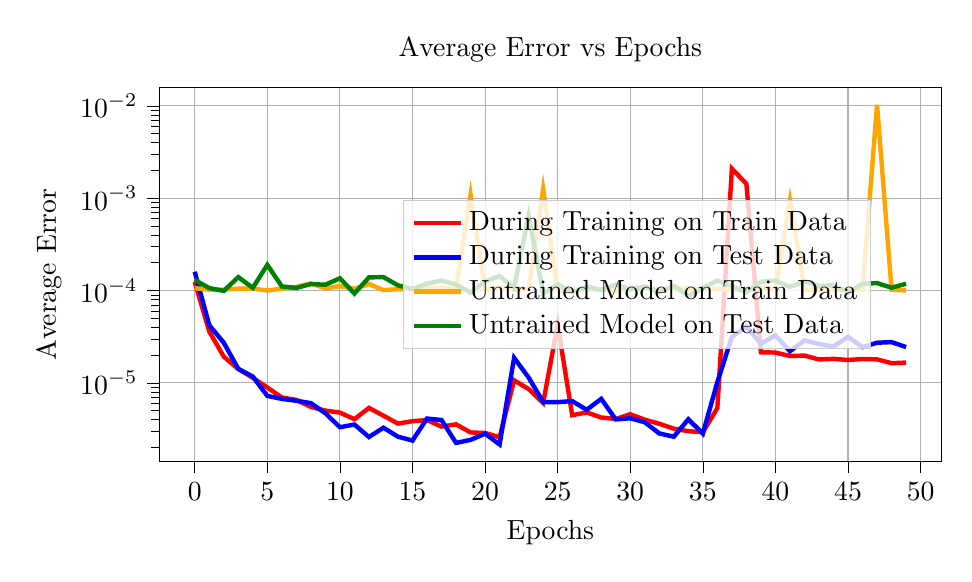
\begin{tikzpicture}

  \definecolor{darkgray176}{RGB}{176,176,176}
  \definecolor{green}{RGB}{0,128,0}
  \definecolor{lightgray204}{RGB}{204,204,204}
  \definecolor{orange}{RGB}{255,165,0}
  
  \begin{axis}[
    width = 0.95\textwidth,
    height = 18em,
  legend cell align={left},
  legend style={
    fill opacity=0.8,
    draw opacity=1,
    text opacity=1,
    at={(0.91,0.5)},
    anchor=east,
    draw=lightgray204
  },
  % log basis y={10},
  tick align=outside,
  tick pos=left,
  title={Average Error vs Epochs},
  x grid style={darkgray176},
  xlabel={Epochs},
  xmajorgrids,
  xmin=-2.45, xmax=51.45,
  xtick style={color=black},
  y grid style={darkgray176},
  ylabel={Average Error},
  ymajorgrids,
  ymin=1.41019431670876e-06, ymax=0.0156679028372775,
ymode=log,
ytick style={color=black},
ytick={1e-07,1e-06,1e-05,0.0001,0.001,0.01,0.1,1},
yticklabels={
  \(\displaystyle {10^{-7}}\),
  \(\displaystyle {10^{-6}}\),
  \(\displaystyle {10^{-5}}\),
  \(\displaystyle {10^{-4}}\),
  \(\displaystyle {10^{-3}}\),
  \(\displaystyle {10^{-2}}\),
  \(\displaystyle {10^{-1}}\),
  \(\displaystyle {10^{0}}\)
}
]
\addplot [ultra thick, red]
table {%
0 0.000123712976346724
1 3.61038109986112e-05
2 1.92390634765616e-05
3 1.41538657771889e-05
4 1.13604182843119e-05
5 8.92032585397828e-06
6 6.95451308274642e-06
7 6.54458608551067e-06
8 5.49529750060174e-06
9 5.00813484904938e-06
10 4.76973809782066e-06
11 4.04770207751426e-06
12 5.36180505150696e-06
13 4.41644124293816e-06
14 3.62722039426444e-06
15 3.85068142350065e-06
16 3.96022960558184e-06
17 3.36456196237123e-06
18 3.55754809788777e-06
19 2.90803609459545e-06
20 2.87022248812718e-06
21 2.58148497778166e-06
22 1.06573234006646e-05
23 8.58057410368929e-06
24 6.06654930379591e-06
25 4.27468585257884e-05
26 4.46790727437474e-06
27 4.7897374315653e-06
28 4.21980212195194e-06
29 4.066063411301e-06
30 4.57945770904189e-06
31 3.99971031583846e-06
32 3.61184743269405e-06
33 3.19425089401193e-06
34 3.00034366773616e-06
35 2.92300092041842e-06
36 5.33908041688846e-06
37 0.00208666943944991
38 0.00143341324292123
39 2.14575902646175e-05
40 2.13133171200752e-05
41 1.95563334273174e-05
42 1.97702920559095e-05
43 1.79422713699751e-05
44 1.8209120753454e-05
45 1.77225774677936e-05
46 1.8146803995478e-05
47 1.79904764081584e-05
48 1.63504064403242e-05
49 1.66026311489986e-05
};
\addlegendentry{During Training on Train Data}
\addplot [ultra thick, blue]
table {%
0 0.000159875882673077
1 4.22315242758486e-05
2 2.7227884856984e-05
3 1.42017352118273e-05
4 1.17081235657679e-05
5 7.23542916603037e-06
6 6.71077714287094e-06
7 6.40759981251904e-06
8 6.03867511017597e-06
9 4.69222231913591e-06
10 3.31214664583968e-06
11 3.5421453503659e-06
12 2.59482339970418e-06
13 3.2733794341766e-06
14 2.61443551607954e-06
15 2.37594713325961e-06
16 4.11221253671101e-06
17 3.96487075704499e-06
18 2.23926417675102e-06
19 2.41555221691669e-06
20 2.8177416879771e-06
21 2.15365366784681e-06
22 1.87013902177569e-05
23 1.14274735096842e-05
24 6.2057692957751e-06
25 6.19489219388925e-06
26 6.35293827144778e-06
27 5.11537382408278e-06
28 6.72031046633492e-06
29 4.02510841013282e-06
30 4.13926454712055e-06
31 3.74754449694592e-06
32 2.83836811831861e-06
33 2.61320633399009e-06
34 4.03772992285667e-06
35 2.82361907011364e-06
36 1.0201881195826e-05
37 3.15313627652358e-05
38 4.07302868552506e-05
39 2.65761373157147e-05
40 3.26319495798089e-05
41 2.20370038732653e-05
42 2.89441613858799e-05
43 2.63891542999772e-05
44 2.47493626375217e-05
45 3.15998440783005e-05
46 2.43979666265659e-05
47 2.72413453785703e-05
48 2.76492264674744e-05
49 2.44446182477986e-05
};
\addlegendentry{During Training on Test Data}
\addplot [ultra thick, orange]
table {%
0 0.000106271909317002
1 0.000102229292679112
2 0.00010267308971379
3 0.000104742110124789
4 0.000105179497040808
5 0.000100018667581026
6 0.000104978236777242
7 0.000109515276562888
8 0.000119890522910282
9 0.000105556289781816
10 0.000111739653220866
11 0.000104603088402655
12 0.000117901385237928
13 0.00010120128717972
14 0.000103505786682945
15 0.000103618745924905
16 0.000106016705103684
17 0.00010689883492887
18 0.000104009690403473
19 0.00109088909812272
20 0.000103115293313749
21 0.00010907154501183
22 0.000102108948340174
23 0.000103274433058687
24 0.00125256320461631
25 9.92863351712003e-05
26 0.000102455873275176
27 0.000102277525002137
28 0.000102194979263004
29 9.96877497527748e-05
30 0.000105364371847827
31 0.000111033332359511
32 0.000102558151411358
33 0.000106491075712256
34 0.000105227059975732
35 0.00010441130871186
36 0.000104104678030126
37 0.00010139533696929
38 0.000101719553640578
39 0.000106533829239197
40 0.000102680489362683
41 0.00094377517234534
42 0.000102259968116414
43 0.00010156721691601
44 0.000102538957435172
45 0.000101136916782707
46 0.000101828067272436
47 0.010259211063385
48 0.000102150734164752
49 0.000100222190667409
};
\addlegendentry{Untrained Model on Train Data}
\addplot [ultra thick, green]
table {%
0 0.000130604763398878
1 0.000106325744127389
2 9.91808701655827e-05
3 0.000139764888444915
4 0.000106910294562113
5 0.000189925674931146
6 0.00011083425488323
7 0.000106884399428964
8 0.000117591385787819
9 0.000115719740279019
10 0.000135850379592739
11 9.29285524762236e-05
12 0.000138900868478231
13 0.000139856783789583
14 0.000113880254502874
15 0.000103845428384375
16 0.000118751777336001
17 0.000128611776744947
18 0.00011601863661781
19 9.52845075516962e-05
20 0.00012534690904431
21 0.000143454322824255
22 0.000107589636172634
23 0.000650533998850733
24 9.27244473132305e-05
25 0.000116712952149101
26 9.58258606260642e-05
27 0.000110465756733902
28 0.000101411693322007
29 0.000116058603452984
30 0.000102887766843196
31 0.0001104218463297
32 9.6138333901763e-05
33 0.000112641544546932
34 8.6982901848387e-05
35 0.000106365303508937
36 0.000128128056530841
37 0.000112121822894551
38 9.54371644183993e-05
39 0.000124593556392938
40 0.000128446350572631
41 0.000109284628706519
42 0.000125934908282943
43 0.000112414883915335
44 0.00011437434295658
45 9.45309875532985e-05
46 0.000118598167318851
47 0.000120423108455725
48 0.000107457301055547
49 0.000118399308121298
};
\addlegendentry{Untrained Model on Test Data}
\end{axis}

\end{tikzpicture}
}\\  
  \subfloat[Proposed Scenario Using Optuna\cite{Akiba2019}: Different Scalars Plus a Single Semi-Positive Definite Matrix$(\tau_k\boldsymbol{S})$, $lr=8.798\times10^{-3}$]{% This file was created with tikzplotlib v0.10.1.
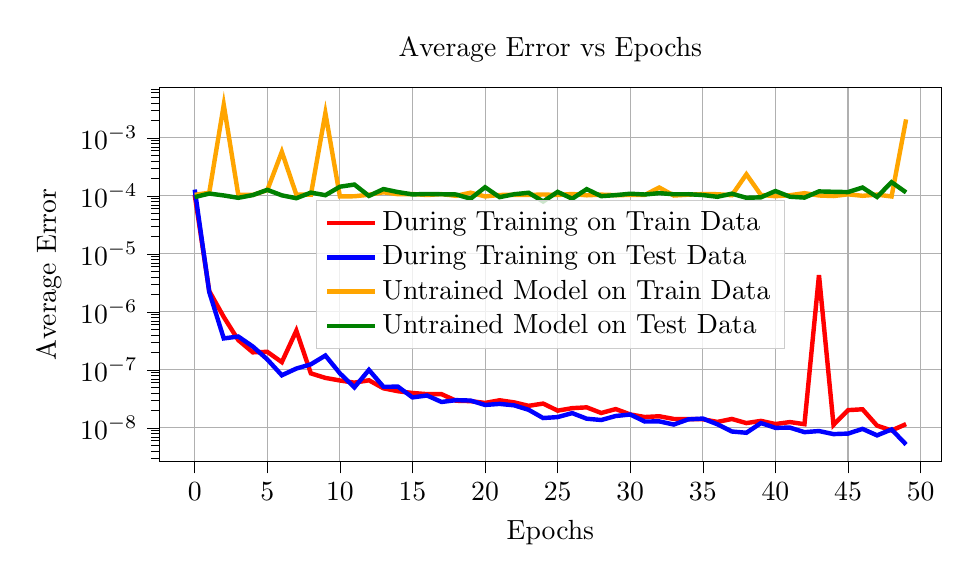
\begin{tikzpicture}

    \definecolor{darkgray176}{RGB}{176,176,176}
    \definecolor{green}{RGB}{0,128,0}
    \definecolor{lightgray204}{RGB}{204,204,204}
    \definecolor{orange}{RGB}{255,165,0}
    
    \begin{axis}[
      width = 0.95\textwidth,
      height = 18em,
    legend cell align={left},
    legend style={
      fill opacity=0.8,
      draw opacity=1,
      text opacity=1,
      at={(0.5,0.5)},
      anchor=center,
      draw=lightgray204
    },
    % log basis y={10},
    tick align=outside,
    tick pos=left,
    title={Average Error vs Epochs},
    x grid style={darkgray176},
    xlabel={Epochs},
    xmajorgrids,
    xmin=-2.45, xmax=51.45,
    xtick style={color=black},
    y grid style={darkgray176},
    ylabel={Average Error},
    ymajorgrids,
    ymin=2.63604330184737e-09, ymax=0.00725950156863836,
    ymode=log,
    ytick style={color=black},
    ytick={1e-10,1e-09,1e-08,1e-07,1e-06,1e-05,0.0001,0.001,0.01,0.1},
    yticklabels={
      \(\displaystyle {10^{-10}}\),
      \(\displaystyle {10^{-9}}\),
      \(\displaystyle {10^{-8}}\),
      \(\displaystyle {10^{-7}}\),
      \(\displaystyle {10^{-6}}\),
      \(\displaystyle {10^{-5}}\),
      \(\displaystyle {10^{-4}}\),
      \(\displaystyle {10^{-3}}\),
      \(\displaystyle {10^{-2}}\),
      \(\displaystyle {10^{-1}}\)
    }
    ]
    \addplot [ultra thick, red]
    table {%
    0 0.000104205340903718
    1 2.2795081804361e-06
    2 8.16013880466926e-07
    3 3.26127519656438e-07
    4 2.00797316551871e-07
    5 2.04524624791702e-07
    6 1.36023288632714e-07
    7 4.74071129019649e-07
    8 8.70571454925084e-08
    9 7.27430773395099e-08
    10 6.5652713487907e-08
    11 6.02018914719338e-08
    12 6.61969394855078e-08
    13 4.81310458155804e-08
    14 4.2873633532281e-08
    15 3.99703772302473e-08
    16 3.81714855279824e-08
    17 3.8142367486671e-08
    18 2.93974711240708e-08
    19 2.89232531258676e-08
    20 2.69239741612637e-08
    21 2.99225142441628e-08
    22 2.75352860512612e-08
    23 2.4009436216943e-08
    24 2.62635957426482e-08
    25 1.98318286237509e-08
    26 2.18844142807484e-08
    27 2.25979448487124e-08
    28 1.80841581709501e-08
    29 2.10961470514803e-08
    30 1.70547433953061e-08
    31 1.53920822754117e-08
    32 1.58656572324389e-08
    33 1.42510874212576e-08
    34 1.41820661880843e-08
    35 1.4081289023693e-08
    36 1.26731078964326e-08
    37 1.42557086135753e-08
    38 1.21001750841288e-08
    39 1.32015909315442e-08
    40 1.16595693100408e-08
    41 1.26017134505219e-08
    42 1.15926468424732e-08
    43 4.30966929343413e-06
    44 1.12703659738145e-08
    45 2.02334238252888e-08
    46 2.09316262100856e-08
    47 1.09466631315058e-08
    48 9.01701913136321e-09
    49 1.16273870531813e-08
    };
    \addlegendentry{During Training on Train Data}
    \addplot [ultra thick, blue]
    table {%
    0 0.000128205894725397
    1 2.19211028706923e-06
    2 3.48693362184349e-07
    3 3.7564521448985e-07
    4 2.53075398859437e-07
    5 1.51381684077023e-07
    6 8.07240780886787e-08
    7 1.05399159622266e-07
    8 1.24686110325456e-07
    9 1.76708667254388e-07
    10 8.71838210514397e-08
    11 4.9951530911585e-08
    12 9.98501263893559e-08
    13 5.1198544070985e-08
    14 5.13218765263446e-08
    15 3.35316165944732e-08
    16 3.61962158024198e-08
    17 2.79910761236124e-08
    18 3.00771283434642e-08
    19 2.95923321402825e-08
    20 2.4853880731257e-08
    21 2.59286903059319e-08
    22 2.44853541886414e-08
    23 2.05111181372786e-08
    24 1.47937218031302e-08
    25 1.5353929683215e-08
    26 1.79923898002698e-08
    27 1.44036702565131e-08
    28 1.36676279183234e-08
    29 1.603949861817e-08
    30 1.70154574874459e-08
    31 1.28716752811897e-08
    32 1.29476260823935e-08
    33 1.14277387552875e-08
    34 1.4037178530657e-08
    35 1.44796095113975e-08
    36 1.15444818149513e-08
    37 8.66101146357323e-09
    38 8.24099988250282e-09
    39 1.21144925202543e-08
    40 1.00226200672182e-08
    41 1.01044204114942e-08
    42 8.44652703335669e-09
    43 8.82723494299853e-09
    44 7.81588394005439e-09
    45 7.98052735007104e-09
    46 9.61182422543061e-09
    47 7.4352684009682e-09
    48 9.4029859454281e-09
    49 5.17222886742275e-09
    };
    \addlegendentry{During Training on Test Data}
    \addplot [ultra thick, orange]
    table {%
    0 0.000104004502645694
    1 0.000113090267404914
    2 0.00369982863776386
    3 0.000103595812106505
    4 0.000103680438769516
    5 0.000125327438581735
    6 0.000573276192881167
    7 0.000104799939435907
    8 0.000104467922938056
    9 0.00266967760398984
    10 9.74361173575744e-05
    11 9.83515856205486e-05
    12 0.000104475227999501
    13 0.000115149639896117
    14 0.000106749808765016
    15 0.000107450287032407
    16 0.000103390899312217
    17 0.000107067287899554
    18 0.000100105462479405
    19 0.000113200912892353
    20 9.77006420725957e-05
    21 0.000103448765003122
    22 0.000104000508144964
    23 0.000103353981103282
    24 0.000105591047031339
    25 0.000103221151221078
    26 0.00010765408660518
    27 0.000102091478765942
    28 0.000104882899904624
    29 0.000102825011708774
    30 0.000103528509498574
    31 0.000103895661595743
    32 0.000138981064083055
    33 0.000101232988527045
    34 0.000104792459751479
    35 0.000107034466054756
    36 0.000106611536466517
    37 0.000102448932011612
    38 0.000235152678214945
    39 0.000103626218333375
    40 9.85821752692573e-05
    41 0.000102437457826454
    42 0.000111155663034879
    43 0.000101380828709807
    44 9.91987908491865e-05
    45 0.000106175990367774
    46 0.000100137636763975
    47 0.000104896309494507
    48 9.75669390754774e-05
    49 0.00207684771157801
    };
    \addlegendentry{Untrained Model on Train Data}
    \addplot [ultra thick, green]
    table {%
    0 9.51192560023628e-05
    1 0.000109474291093647
    2 0.000101536650618073
    3 9.24414925975725e-05
    4 0.000102999874798115
    5 0.000126819082652219
    6 0.000101982383057475
    7 9.10065864445642e-05
    8 0.000113746289571282
    9 0.000102590936876368
    10 0.000143659664900042
    11 0.000156529058585875
    12 9.96770613710396e-05
    13 0.000130805958178826
    14 0.000116074705147184
    15 0.000105866813100874
    16 0.000107682615634985
    17 0.000106509614852257
    18 0.000105575592897367
    19 8.92794705578126e-05
    20 0.000140646734507754
    21 9.49161913013086e-05
    22 0.000106560277345125
    23 0.000113010035420302
    24 7.99219124019146e-05
    25 0.00011702597112162
    26 8.920714026317e-05
    27 0.000130467757117003
    28 9.88191241049208e-05
    29 0.000102830796095077
    30 0.000108744738099631
    31 0.000105451188574079
    32 0.000111337336420547
    33 0.000106409403088037
    34 0.000106660001620185
    35 0.000103220765595324
    36 9.62638878263533e-05
    37 0.000108933658339083
    38 9.25103668123484e-05
    39 9.42573096835986e-05
    40 0.000121093005873263
    41 9.66605221037753e-05
    42 9.32564653339796e-05
    43 0.000119190364785027
    44 0.000117450043035205
    45 0.0001160800238722
    46 0.000139031486469321
    47 9.57154188654386e-05
    48 0.000171932319062762
    49 0.000114621827378869
    };
    \addlegendentry{Untrained Model on Test Data}
    \end{axis}
    
    \end{tikzpicture}
    }\\  
  \caption{Training the \ac{UWF} Algorithm in different Scenarios With and Without Optuna\cite{Akiba2019}}
  \label{fig:uwf_training_07_08_optuna}
  \end{figure}
%   \clearpage % End the page
}
%%%%%%%%%%%%%%%%%%%%%%%%%%%%%%%%%%%%%%%%%%%%%%%%%%%%%%%%%%%%%
%%%%% Training URWF Without Hyperparameter Optimization %%%%%%
%%%%%%%%%%%%%%%%%%%%%%%%%%%%%%%%%%%%%%%%%%%%%%%%%%%%%%%%%%%%%
\afterpage{%
%   \clearpage % Start a new page
\begin{figure}[!htbp]
  \subfloat[Single Scalar$(\tau)$]{% This file was created with tikzplotlib v0.10.1.
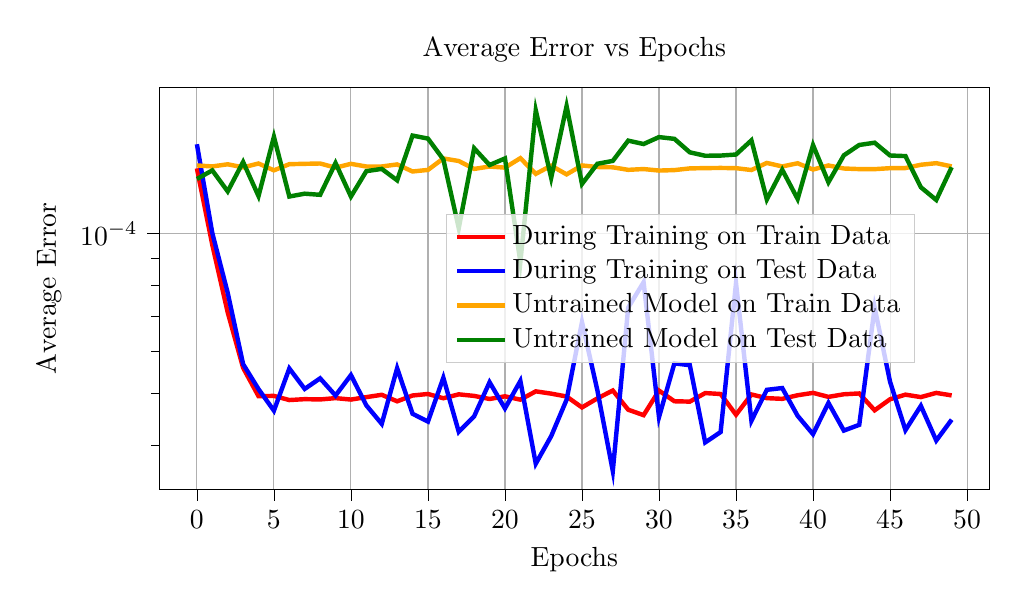
\begin{tikzpicture}

  \definecolor{darkgray176}{RGB}{176,176,176}
  \definecolor{green}{RGB}{0,128,0}
  \definecolor{lightgray204}{RGB}{204,204,204}
  \definecolor{orange}{RGB}{255,165,0}
  
  \begin{axis}[
    width = 1.0\textwidth,
    height = 19em,
  legend cell align={left},
  legend style={
    fill opacity=0.8,
    draw opacity=1,
    text opacity=1,
    at={(0.91,0.5)},
    anchor=east,
    draw=lightgray204
  },
  % log basis y={10},
  tick align=outside,
  tick pos=left,
  title={Average Error vs Epochs},
  x grid style={darkgray176},
  xlabel={Epochs},
  xmajorgrids,
  xmin=-2.45, xmax=51.45,
  xtick style={color=black},
  y grid style={darkgray176},
  ylabel={Average Error},
  ymajorgrids,
  ymin=3.30722135247185e-05, ymax=0.000188104234714924,
  ymode=log,
  ytick style={color=black},
  ytick={1e-06,1e-05,0.0001,0.001,0.01},
  yticklabels={
    \(\displaystyle {10^{-6}}\),
    \(\displaystyle {10^{-5}}\),
    \(\displaystyle {10^{-4}}\),
    \(\displaystyle {10^{-3}}\),
    \(\displaystyle {10^{-2}}\)
  }
  ]
  \addplot [ultra thick, red]
  table {%
  0 0.000132722096168436
  1 9.52958143898286e-05
  2 7.11312095518224e-05
  3 5.59525251446757e-05
  4 4.94734194944613e-05
  5 4.95356325700413e-05
  6 4.86540520796552e-05
  7 4.88426849187817e-05
  8 4.87789220642298e-05
  9 4.90620986965951e-05
  10 4.87564029754139e-05
  11 4.92705366923474e-05
  12 4.97732726216782e-05
  13 4.83878284285311e-05
  14 4.96224929520395e-05
  15 4.99510824738536e-05
  16 4.90340717078652e-05
  17 4.98722329211887e-05
  18 4.95317617605906e-05
  19 4.88754849357065e-05
  20 4.94462146889418e-05
  21 4.87317229271866e-05
  22 5.05235257151071e-05
  23 5.0024245865643e-05
  24 4.94094638270326e-05
  25 4.71192179247737e-05
  26 4.90080456074793e-05
  27 5.07079239469022e-05
  28 4.66571473225486e-05
  29 4.55734552815557e-05
  30 5.06827636854723e-05
  31 4.83968869957607e-05
  32 4.83256881125271e-05
  33 5.0144979468314e-05
  34 4.99464476888534e-05
  35 4.56594752904493e-05
  36 4.98443841934204e-05
  37 4.90569836983923e-05
  38 4.89077756355982e-05
  39 4.96737193316221e-05
  40 5.01869035360869e-05
  41 4.93312109028921e-05
  42 4.98860681545921e-05
  43 5.00653732160572e-05
  44 4.65431585325859e-05
  45 4.88188707095105e-05
  46 4.98049921588972e-05
  47 4.92811013828032e-05
  48 5.01822796650231e-05
  49 4.96389002364594e-05
  };
  \addlegendentry{During Training on Train Data}
  \addplot [ultra thick, blue]
  table {%
  0 0.000147356346133165
  1 0.000100276833109092
  2 7.74033032939769e-05
  3 5.68429713894147e-05
  4 5.10137870151084e-05
  5 4.64688382635359e-05
  6 5.57806524739135e-05
  7 5.1057828386547e-05
  8 5.34521313966252e-05
  9 4.96142783958931e-05
  10 5.42103043699171e-05
  11 4.7545585402986e-05
  12 4.38857059634756e-05
  13 5.58492865820881e-05
  14 4.58449612779077e-05
  15 4.43196513515431e-05
  16 5.35876279172953e-05
  17 4.23945093643852e-05
  18 4.53545399068389e-05
  19 5.25535251654219e-05
  20 4.69236656499561e-05
  21 5.28460477653425e-05
  22 3.69406589015853e-05
  23 4.16071488871239e-05
  24 4.87198121845722e-05
  25 6.8199158704374e-05
  26 5.0729689974105e-05
  27 3.57913850166369e-05
  28 7.26350262993947e-05
  29 8.1043537647929e-05
  30 4.51905725640245e-05
  31 5.70314368815161e-05
  32 5.65893242310267e-05
  33 4.04946149501484e-05
  34 4.23562341893557e-05
  35 8.07066462584771e-05
  36 4.44882716692518e-05
  37 5.08558587171137e-05
  38 5.12504157086369e-05
  39 4.54418550361879e-05
  40 4.19671923737042e-05
  41 4.80627386423294e-05
  42 4.26279038947541e-05
  43 4.37011694884859e-05
  44 7.25988211343065e-05
  45 5.26790354342666e-05
  46 4.27131417382043e-05
  47 4.74478620162699e-05
  48 4.08320811402518e-05
  49 4.46896556240972e-05
  };
  \addlegendentry{During Training on Test Data}
  \addplot [ultra thick, orange]
  table {%
  0 0.000134415182401426
  1 0.000133859735797159
  2 0.000135096372105181
  3 0.000133315537823364
  4 0.000135558802867308
  5 0.000131604872876778
  6 0.000135166221298277
  7 0.000135371694341302
  8 0.00013555760961026
  9 0.000133147303131409
  10 0.000135355425300077
  11 0.000133816851302981
  12 0.00013382603356149
  13 0.000135015754494816
  14 0.000130949250888079
  15 0.000131850087200291
  16 0.000138567527756095
  17 0.000137042501592077
  18 0.000132412038510665
  19 0.000133806184749119
  20 0.00013315056276042
  21 0.000138728239107877
  22 0.000129598542116582
  23 0.000134296817122959
  24 0.000129316467791796
  25 0.000134426998556592
  26 0.000133511028252542
  27 0.000133338689920492
  28 0.000131890992633998
  29 0.000132342014694586
  30 0.000131475171656348
  31 0.000131742417579517
  32 0.000132709450554103
  33 0.000132882501929998
  34 0.000132975561427884
  35 0.0001328465732513
  36 0.000131782973767258
  37 0.000135892565594986
  38 0.000133842084323987
  39 0.000135688576847315
  40 0.000132072207634337
  41 0.000134420246467926
  42 0.000132650457089767
  43 0.000132311062770896
  44 0.000132282293634489
  45 0.000132839733851142
  46 0.00013292086077854
  47 0.00013482163194567
  48 0.000135752008645795
  49 0.000133861845824867
  };
  \addlegendentry{Untrained Model on Train Data}
  \addplot [ultra thick, green]
  table {%
  0 0.00012677519407589
  1 0.000131578868604265
  2 0.000120126052934211
  3 0.000136456466862001
  4 0.000117726136522833
  5 0.000152216060087085
  6 0.000117487055831589
  7 0.000118944961286616
  8 0.000118362011562567
  9 0.000135828202473931
  10 0.000117471114208456
  11 0.000131132823298685
  12 0.0001324288896285
  13 0.00012603857612703
  14 0.000153000306454487
  15 0.000151011321577244
  16 0.000137982569867745
  17 0.000102457801403943
  18 0.000144789562909864
  19 0.0001346626522718
  20 0.00013855162251275
  21 8.84784312802367e-05
  22 0.000170658269780688
  23 0.000127359642647207
  24 0.000173813430592418
  25 0.000124067300930619
  26 0.000135398469865322
  27 0.000137087437906303
  28 0.00014967487368267
  29 0.000147490325616673
  30 0.000151992935570888
  31 0.000150832158396952
  32 0.000142279764986597
  33 0.000140183008625172
  34 0.000140295756864361
  35 0.000140935080708005
  36 0.000149868414155208
  37 0.000115996052045375
  38 0.000131940701976418
  39 0.000116244016680866
  40 0.000146826612763107
  41 0.000124963815324008
  42 0.000140456089866348
  43 0.000146886712173
  44 0.000148353181430139
  45 0.000140342046506703
  46 0.000139979019877501
  47 0.000122307494166307
  48 0.000115747614472639
  49 0.000133389243273996
  };
  \addlegendentry{Untrained Model on Test Data}
  \end{axis}
  
  \end{tikzpicture}
  }\\
  \subfloat[Different Scalars$(\tau_k)$]{% This file was created with tikzplotlib v0.10.1.
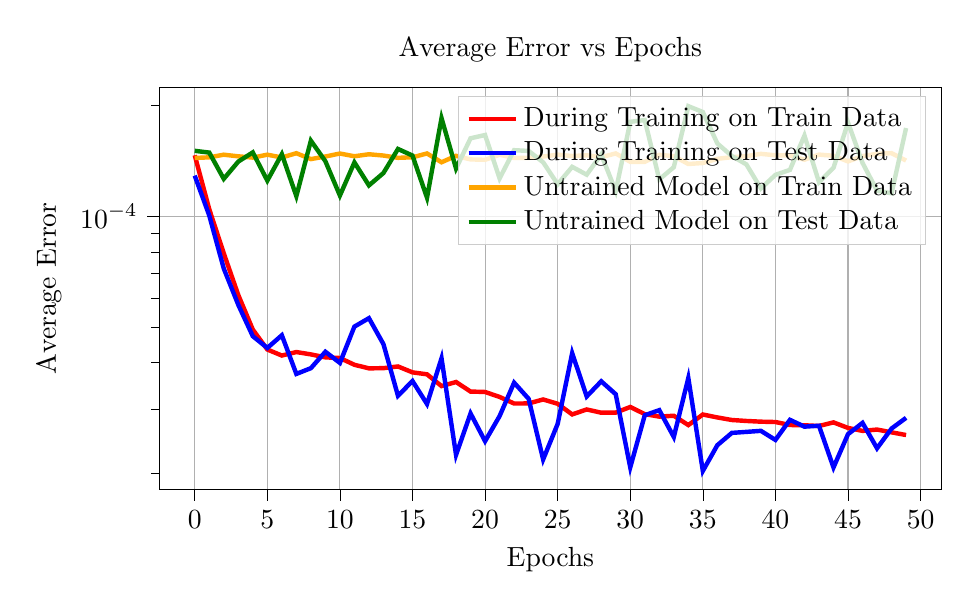
\begin{tikzpicture}

    \definecolor{darkgray176}{RGB}{176,176,176}
    \definecolor{green}{RGB}{0,128,0}
    \definecolor{lightgray204}{RGB}{204,204,204}
    \definecolor{orange}{RGB}{255,165,0}
    
    \begin{axis}[
      width = 0.95\textwidth,
      height = 19em,
    legend cell align={left},
    legend style={
      fill opacity=0.8,
      draw opacity=1,
      text opacity=1,
      % at={(0.91,0.5)},
      % anchor=east,
      draw=lightgray204
    },
    % log basis y={10},
    tick align=outside,
    tick pos=left,
    title={Average Error vs Epochs},
    x grid style={darkgray176},
    xlabel={Epochs},
    xmajorgrids,
    xmin=-2.45, xmax=51.45,
    xtick style={color=black},
    y grid style={darkgray176},
    ylabel={Average Error},
    ymajorgrids,
    ymin=1.81602095355054e-05, ymax=0.000222783350611656,
    ymode=log,
    ytick style={color=black},
    ytick={1e-06,1e-05,0.0001,0.001,0.01},
    yticklabels={
      \(\displaystyle {10^{-6}}\),
      \(\displaystyle {10^{-5}}\),
      \(\displaystyle {10^{-4}}\),
      \(\displaystyle {10^{-3}}\),
      \(\displaystyle {10^{-2}}\)
    }
    ]
    \addplot [ultra thick, red]
    table {%
    0 0.000146278194733895
    1 0.000104420905699953
    2 7.92681239545345e-05
    3 6.10758288530633e-05
    4 4.92224680783693e-05
    5 4.34550092904828e-05
    6 4.18473209720105e-05
    7 4.27740997110959e-05
    8 4.21492586610839e-05
    9 4.13740053772926e-05
    10 4.12062763643917e-05
    11 3.95096503780223e-05
    12 3.86323808925226e-05
    13 3.8685386243742e-05
    14 3.90951099689119e-05
    15 3.7674093618989e-05
    16 3.72231625078712e-05
    17 3.45841617672704e-05
    18 3.54710755345877e-05
    19 3.34202304657083e-05
    20 3.33290299749933e-05
    21 3.23112872138154e-05
    22 3.10100913338829e-05
    23 3.1028324883664e-05
    24 3.18035745294765e-05
    25 3.09636925521772e-05
    26 2.89666477328865e-05
    27 2.98817540169694e-05
    28 2.92815784632694e-05
    29 2.92987824650481e-05
    30 3.03483375319047e-05
    31 2.90223379124654e-05
    32 2.85742298729019e-05
    33 2.87294860754628e-05
    34 2.71037642960437e-05
    35 2.89524341496872e-05
    36 2.84268226096174e-05
    37 2.79751275229501e-05
    38 2.78087027254514e-05
    39 2.76841983577469e-05
    40 2.76240880339174e-05
    41 2.71164917649003e-05
    42 2.70670807367424e-05
    43 2.69537595158909e-05
    44 2.75629245152231e-05
    45 2.6622759833117e-05
    46 2.61352506640833e-05
    47 2.63559304585215e-05
    48 2.59002445091028e-05
    49 2.54677142947912e-05
    };
    \addlegendentry{During Training on Train Data}
    \addplot [ultra thick, blue]
    table {%
    0 0.000128779443912208
    1 0.00010038409527624
    2 7.20859316061251e-05
    3 5.74429686821532e-05
    4 4.72210740554146e-05
    5 4.38880924775731e-05
    6 4.74986336485017e-05
    7 3.7310368497856e-05
    8 3.86739084206056e-05
    9 4.2848852899624e-05
    10 3.9968599594431e-05
    11 5.0143735279562e-05
    12 5.285011138767e-05
    13 4.49300969194155e-05
    14 3.25484543282073e-05
    15 3.56887139787432e-05
    16 3.09173701680265e-05
    17 4.11355395044666e-05
    18 2.24964205699507e-05
    19 2.91467531496892e-05
    20 2.45067039941205e-05
    21 2.86695176328067e-05
    22 3.53258474206086e-05
    23 3.19383507303428e-05
    24 2.18671866605291e-05
    25 2.73038804152748e-05
    26 4.2485826270422e-05
    27 3.24111788359005e-05
    28 3.56320124410558e-05
    29 3.28617716149893e-05
    30 2.08107903745258e-05
    31 2.8820493753301e-05
    32 2.97523602057481e-05
    33 2.5161634766846e-05
    34 3.63602011930197e-05
    35 2.03521376533899e-05
    36 2.3903059627628e-05
    37 2.58119016507408e-05
    38 2.59747375821462e-05
    39 2.61434706771979e-05
    40 2.47025800490519e-05
    41 2.80039475910598e-05
    42 2.68369312834693e-05
    43 2.69887150352588e-05
    44 2.07989851332968e-05
    45 2.56072144111386e-05
    46 2.74763297056779e-05
    47 2.34442468354246e-05
    48 2.65273101831554e-05
    49 2.83582612610189e-05
    };
    \addlegendentry{During Training on Test Data}
    \addplot [ultra thick, orange]
    table {%
    0 0.000143817727803253
    1 0.000144362973514944
    2 0.000146766687976196
    3 0.000145289624924771
    4 0.000144115459988825
    5 0.000146782738738693
    6 0.000144232981256209
    7 0.000148136517964303
    8 0.000142785676871426
    9 0.000145113124744967
    10 0.000147847051266581
    11 0.000145348269143142
    12 0.000147180369822308
    13 0.000145986239658669
    14 0.000143930912599899
    15 0.000144404504681006
    16 0.000147901533637196
    17 0.000139990574098192
    18 0.000145746729685925
    19 0.000142500211950392
    20 0.000142163597047329
    21 0.000146696082083508
    22 0.00014386406110134
    23 0.000143894605571404
    24 0.000145068916026503
    25 0.000146825681440532
    26 0.000145544589031488
    27 0.000146261707413942
    28 0.000144508856465109
    29 0.000147926708450541
    30 0.000140387055580504
    31 0.000140381875098683
    32 0.00014663758338429
    33 0.00014546888996847
    34 0.000138474060804583
    35 0.000139353855047375
    36 0.000143018041853793
    37 0.000144513905979693
    38 0.000145408208481967
    39 0.00014754910080228
    40 0.000146216785651632
    41 0.000146020873216912
    42 0.000142244753078558
    43 0.000146861115354113
    44 0.000145769605296664
    45 0.000140737523906864
    46 0.000145486628753133
    47 0.000147612619912252
    48 0.000148156919749454
    49 0.000141483877087012
    };
    \addlegendentry{Untrained Model on Train Data}
    \addplot [ultra thick, green]
    table {%
    0 0.000150364750879817
    1 0.000148715800605714
    2 0.000126212136819959
    3 0.000140571341034956
    4 0.00014891754835844
    5 0.0001248148328159
    6 0.000147257611388341
    7 0.000113281806989107
    8 0.000160188879817724
    9 0.000140890551847406
    10 0.000113709320430644
    11 0.000139861251227558
    12 0.00012114318087697
    13 0.000130904605612159
    14 0.000152134743984789
    15 0.000145973521284759
    16 0.000112183719465975
    17 0.000184424745384604
    18 0.000134632413391955
    19 0.00016261384007521
    20 0.000165981182362884
    21 0.00012655348109547
    22 0.000150970416143537
    23 0.000150248713907786
    24 0.000139949814183637
    25 0.000122067860502284
    26 0.000136034286697395
    27 0.000129538966575637
    28 0.000146950769703835
    29 0.000116940143925603
    30 0.000180271337740123
    31 0.000182227056939155
    32 0.000125736318295822
    33 0.000135748166940175
    34 0.000198789552086964
    35 0.000191611266927794
    36 0.000157448623212986
    37 0.000145551850437187
    38 0.000138119357870892
    39 0.000118853095045779
    40 0.000129383552120999
    41 0.000133493827888742
    42 0.00016541252261959
    43 0.000123607329442166
    44 0.000135195485199802
    45 0.000179384034709074
    46 0.000139412193675525
    47 0.00011720007751137
    48 0.000115313268906903
    49 0.000173394801095128
    };
    \addlegendentry{Untrained Model on Test Data}
    \end{axis}
    
    \end{tikzpicture}
    }\\
  \subfloat[Single Matrix$(\boldsymbol{M})$]{% This file was created with tikzplotlib v0.10.1.
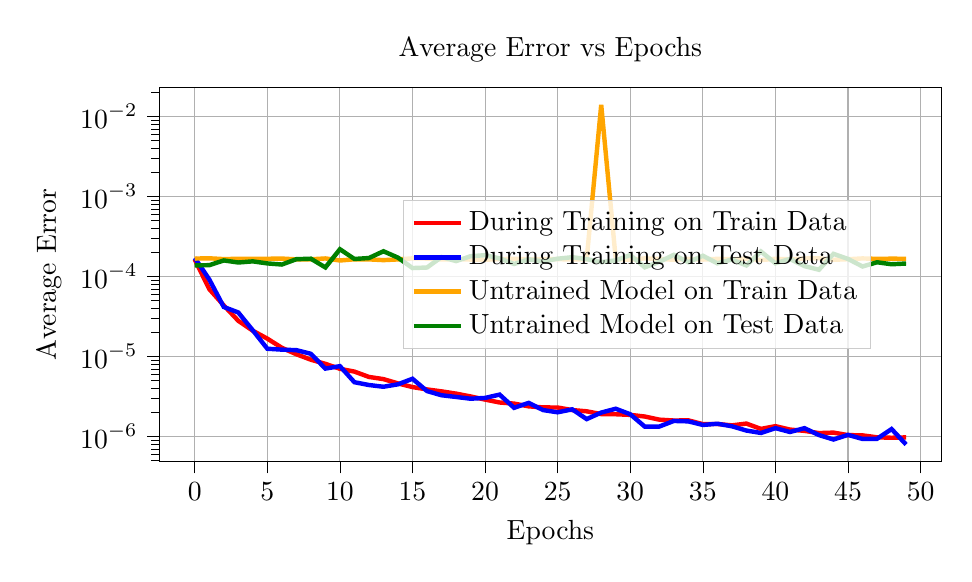
\begin{tikzpicture}

  \definecolor{darkgray176}{RGB}{176,176,176}
  \definecolor{green}{RGB}{0,128,0}
  \definecolor{lightgray204}{RGB}{204,204,204}
  \definecolor{orange}{RGB}{255,165,0}
  
  \begin{axis}[
    width = 0.95\textwidth,
    height = 18em,
  legend cell align={left},
  legend style={
    fill opacity=0.8,
    draw opacity=1,
    text opacity=1,
    at={(0.91,0.5)},
    anchor=east,
    draw=lightgray204
  },
  % log basis y={10},
  tick align=outside,
  tick pos=left,
  title={Average Error vs Epochs},
  x grid style={darkgray176},
  xlabel={Epochs},
  xmajorgrids,
  xmin=-2.45, xmax=51.45,
  xtick style={color=black},
  y grid style={darkgray176},
  ylabel={Average Error},
  ymajorgrids,
  ymin=4.86653883990184e-07, ymax=0.0227388191398161,
  ymode=log,
  ytick style={color=black},
  ytick={1e-08,1e-07,1e-06,1e-05,0.0001,0.001,0.01,0.1,1},
yticklabels={
  \(\displaystyle {10^{-8}}\),
  \(\displaystyle {10^{-7}}\),
  \(\displaystyle {10^{-6}}\),
  \(\displaystyle {10^{-5}}\),
  \(\displaystyle {10^{-4}}\),
  \(\displaystyle {10^{-3}}\),
  \(\displaystyle {10^{-2}}\),
  \(\displaystyle {10^{-1}}\),
  \(\displaystyle {10^{0}}\)
}
  ]
  \addplot [ultra thick, red]
table {%
0 0.000163097938639112
1 6.95640046615154e-05
2 4.34557296102867e-05
3 2.79197738564108e-05
4 2.09615609492175e-05
5 1.66988993441919e-05
6 1.28378760564374e-05
7 1.0652799574018e-05
8 9.10444123292109e-06
9 8.07891319709597e-06
10 7.00679311194108e-06
11 6.46568105366896e-06
12 5.54613734493614e-06
13 5.20814501214772e-06
14 4.60338424090878e-06
15 4.14187388741993e-06
16 3.87155705539044e-06
17 3.66023209608102e-06
18 3.43169858751935e-06
19 3.16300565827987e-06
20 2.88951900984102e-06
21 2.65776702690346e-06
22 2.57361512012722e-06
23 2.38001484831329e-06
24 2.30703153647482e-06
25 2.29981696975301e-06
26 2.13718476516078e-06
27 2.06161598725885e-06
28 1.90302205282933e-06
29 1.89487604984606e-06
30 1.86091483556083e-06
31 1.7752225858203e-06
32 1.62237029144308e-06
33 1.58172042574733e-06
34 1.58960199314606e-06
35 1.42605972541787e-06
36 1.43255817874888e-06
37 1.37571066716191e-06
38 1.44837963489408e-06
39 1.24299731396604e-06
40 1.34513811644865e-06
41 1.21901894090115e-06
42 1.17452839276666e-06
43 1.10200176095532e-06
44 1.11689780624147e-06
45 1.03926151950873e-06
46 1.03192769529414e-06
47 9.74933186626004e-07
48 9.63614297688764e-07
49 9.73476744547952e-07
};
\addlegendentry{During Training on Train Data}
\addplot [ultra thick, blue]
table {%
0 0.000170692641404457
1 9.19459635042585e-05
2 4.15414688177407e-05
3 3.54702751792502e-05
4 2.12094691960374e-05
5 1.24855350804864e-05
6 1.21629809655133e-05
7 1.19845199151314e-05
8 1.07882378870272e-05
9 7.0505338953808e-06
10 7.56783765609725e-06
11 4.76404329674551e-06
12 4.39399946117192e-06
13 4.18000399804441e-06
14 4.48639048045152e-06
15 5.26103758602403e-06
16 3.69247027265374e-06
17 3.27280577039346e-06
18 3.11769122163241e-06
19 2.96365715257707e-06
20 3.03114143207495e-06
21 3.33551702169643e-06
22 2.28128169510455e-06
23 2.62626690528123e-06
24 2.1363327959989e-06
25 2.00401018446428e-06
26 2.18199670598551e-06
27 1.64860466611572e-06
28 1.9884250832547e-06
29 2.22067751565191e-06
30 1.89409990980494e-06
31 1.32749971726298e-06
32 1.33019966597203e-06
33 1.56249666360964e-06
34 1.54365932303335e-06
35 1.39256223974371e-06
36 1.44203693253075e-06
37 1.34115566652326e-06
38 1.18524599201919e-06
39 1.10521705209976e-06
40 1.27091846024996e-06
41 1.1371939763194e-06
42 1.26946542877704e-06
43 1.04059097338904e-06
44 9.16003955353517e-07
45 1.04647676835157e-06
46 9.31057911657263e-07
47 9.34875686198211e-07
48 1.23812992569583e-06
49 7.93363767570554e-07
};
\addlegendentry{During Training on Test Data}
\addplot [ultra thick, orange]
table {%
0 0.000167268663062714
1 0.000168611761182547
2 0.000164750032126904
3 0.000166074707522057
4 0.000165510311489925
5 0.000166329540661536
6 0.000167264486663043
7 0.000163467208039947
8 0.000163789329235442
9 0.000167902631801553
10 0.000158251743414439
11 0.000163772841915488
12 0.000163379823789001
13 0.000159947972861119
14 0.000163212345796637
15 0.000168250291608274
16 0.000167275851708837
17 0.00016272951324936
18 0.000165133300470188
19 0.000162475116667338
20 0.000161717063747346
21 0.000164484881679527
22 0.000166474826983176
23 0.000163901393534616
24 0.00016524524835404
25 0.000164450189913623
26 0.000162684242241085
27 0.000163810182129964
28 0.0139481220394373
29 0.00016462522034999
30 0.000161635733093135
31 0.000168101963936351
32 0.000165689591085538
33 0.000161484422278591
34 0.000165562189067714
35 0.000162491676746868
36 0.000165928257047199
37 0.000164456811035052
38 0.000166921367053874
39 0.000159998307935894
40 0.000166102094226517
41 0.000163806194905192
42 0.000167545396834612
43 0.000168941318406723
44 0.000161504111019894
45 0.000164178913109936
46 0.000167981517734006
47 0.000165818899404258
48 0.000166785175679252
49 0.000166209385497496
};
\addlegendentry{Untrained Model on Train Data}
\addplot [ultra thick, green]
table {%
0 0.000137429335154593
1 0.000138295567012392
2 0.000158476585056633
3 0.000149381274241023
4 0.000154329158249311
5 0.000145530575537123
6 0.000140856049256399
7 0.000164252924150787
8 0.000166630212333985
9 0.000129618609207682
10 0.000218662316910923
11 0.000165390243637376
12 0.000169930906849913
13 0.000206377269933
14 0.00017179134010803
15 0.000127295410493389
16 0.000129273044876754
17 0.000174764529219829
18 0.000155563189764507
19 0.00017893330368679
20 0.00018444396846462
21 0.000167917532962747
22 0.000143270124681294
23 0.000163351345690899
24 0.000153900356963277
25 0.000166609228472225
26 0.000174030355992727
27 0.000164638928254135
28 0.000151140950038098
29 0.000158716487931088
30 0.000185446187970228
31 0.000130001790239476
32 0.000152179549331777
33 0.000186295816092752
34 0.000150395178934559
35 0.000181550378329121
36 0.000145733851240948
37 0.000162864715093747
38 0.00013712968211621
39 0.000205252305022441
40 0.000145977654028684
41 0.000165515957633033
42 0.000134605827042833
43 0.000121332785056438
44 0.00019154827168677
45 0.000165487450431101
46 0.00013320310972631
47 0.000150331645272672
48 0.000142030883580446
49 0.000145056197652593
};
\addlegendentry{Untrained Model on Test Data}
\end{axis}

\end{tikzpicture}}\\  
  \caption{Training the \ac{URWF} Algorithm in different Scenarios Without Optuna\cite{Akiba2019}}
  \label{fig:urwf_training_01_02_03}
  \end{figure}
%   \clearpage % End the page
}
\afterpage{%
%   \clearpage % Start a new page
\begin{figure}[!htbp]
  \subfloat[Single Semi-Positive Definite Matrix$(\boldsymbol{S})$]{% This file was created with tikzplotlib v0.10.1.
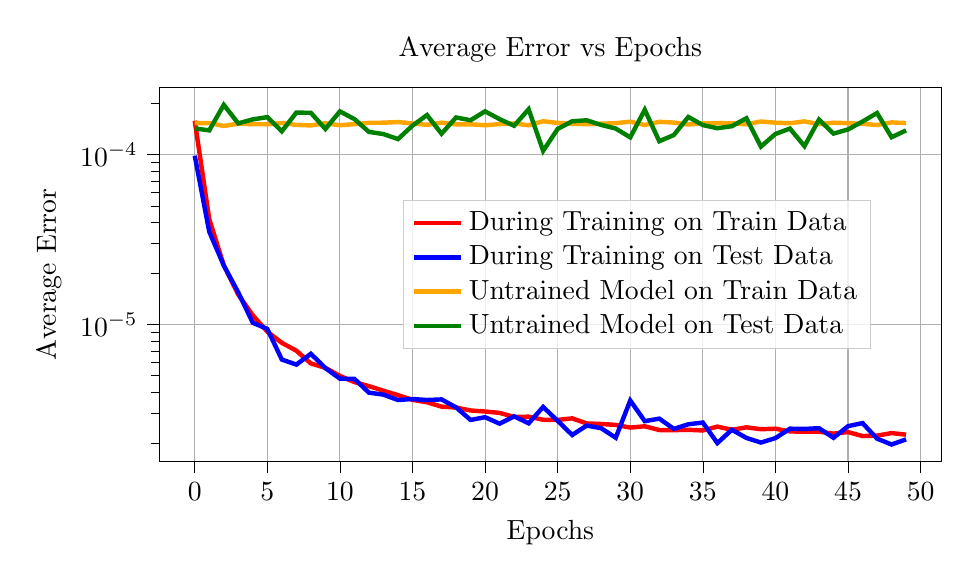
\begin{tikzpicture}

  \definecolor{darkgray176}{RGB}{176,176,176}
  \definecolor{green}{RGB}{0,128,0}
  \definecolor{lightgray204}{RGB}{204,204,204}
  \definecolor{orange}{RGB}{255,165,0}
  
  \begin{axis}[
    width = 0.95\textwidth,
    height = 18em,
  legend cell align={left},
  legend style={
    fill opacity=0.8,
    draw opacity=1,
    text opacity=1,
    at={(0.91,0.5)},
    anchor=east,
    draw=lightgray204
  },
  % log basis y={10},
  tick align=outside,
  tick pos=left,
  title={Average Error vs Epochs},
  x grid style={darkgray176},
  xlabel={Epochs},
  xmajorgrids,
  xmin=-2.45, xmax=51.45,
  xtick style={color=black},
  y grid style={darkgray176},
  ylabel={Average Error},
  ymajorgrids,
  ymin=1.55984612605889e-06, ymax=0.000247681245738091,
ymode=log,
ytick style={color=black},
ytick={1e-07,1e-06,1e-05,0.0001,0.001,0.01},
yticklabels={
  \(\displaystyle {10^{-7}}\),
  \(\displaystyle {10^{-6}}\),
  \(\displaystyle {10^{-5}}\),
  \(\displaystyle {10^{-4}}\),
  \(\displaystyle {10^{-3}}\),
  \(\displaystyle {10^{-2}}\)
}
  ]
  \addplot [ultra thick, red]
table {%
0 0.000158629423822276
1 4.17500705225393e-05
2 2.23410734179197e-05
3 1.49923098433646e-05
4 1.13186724775005e-05
5 9.07615412870655e-06
6 7.79907350079156e-06
7 7.01064618624514e-06
8 5.89603132539196e-06
9 5.5544014685438e-06
10 4.97701785207028e-06
11 4.58103113487596e-06
12 4.33344484918052e-06
13 4.07163042837055e-06
14 3.83643191526062e-06
15 3.59927594217879e-06
16 3.48308049069601e-06
17 3.28366763824306e-06
18 3.24376105709234e-06
19 3.11671965391724e-06
20 3.07204231830838e-06
21 3.01650766232342e-06
22 2.8517763439595e-06
23 2.86554063677613e-06
24 2.74647231890413e-06
25 2.74263447863632e-06
26 2.79981736639456e-06
27 2.61375680565834e-06
28 2.59432090388145e-06
29 2.56180942415085e-06
30 2.47075331571978e-06
31 2.5146134703391e-06
32 2.38996767620847e-06
33 2.38629627347109e-06
34 2.39670816881699e-06
35 2.37572703554179e-06
36 2.50309471994115e-06
37 2.3985255666048e-06
38 2.47841694545059e-06
39 2.41662883126992e-06
40 2.43350336859294e-06
41 2.34371736951289e-06
42 2.33795276471938e-06
43 2.33626451517921e-06
44 2.27647865358449e-06
45 2.32412526202097e-06
46 2.20256538341346e-06
47 2.21448135562241e-06
48 2.2928848011361e-06
49 2.24423251893313e-06
};
\addlegendentry{During Training on Train Data}
\addplot [ultra thick, blue]
table {%
0 9.87597886705771e-05
1 3.5224966268288e-05
2 2.22798680624692e-05
3 1.54417248268146e-05
4 1.02357944342657e-05
5 9.41831694944995e-06
6 6.21941171630169e-06
7 5.80472351430217e-06
8 6.72237501930795e-06
9 5.53433847017004e-06
10 4.79677191833616e-06
11 4.78111951451865e-06
12 3.96789118894958e-06
13 3.8617140489805e-06
14 3.59103978553321e-06
15 3.64064408131526e-06
16 3.59160890184285e-06
17 3.62066725756449e-06
18 3.25107043863682e-06
19 2.74062654170848e-06
20 2.84425550489686e-06
21 2.60542879004788e-06
22 2.87777834273584e-06
23 2.617919108161e-06
24 3.26798544847406e-06
25 2.70756140707817e-06
26 2.23450524572399e-06
27 2.53932171290217e-06
28 2.44782427216705e-06
29 2.15366708289366e-06
30 3.5666532767209e-06
31 2.6958002763422e-06
32 2.78928996522154e-06
33 2.4274806946778e-06
34 2.58378622675082e-06
35 2.64566619989637e-06
36 2.00250156012771e-06
37 2.39911287280847e-06
38 2.14669603337825e-06
39 2.01651187126117e-06
40 2.1419243694254e-06
41 2.43437216340681e-06
42 2.42601004174503e-06
43 2.44980583374854e-06
44 2.15043269236048e-06
45 2.5189995085384e-06
46 2.62520006799605e-06
47 2.1261782876536e-06
48 1.96389669326891e-06
49 2.10574557968357e-06
};
\addlegendentry{During Training on Test Data}
\addplot [ultra thick, orange]
table {%
0 0.000153553526615724
1 0.0001537842763355
2 0.000147777231177315
3 0.00015241838991642
4 0.00015136860019993
5 0.00015115799033083
6 0.000153794055222534
7 0.000149910119944252
8 0.000148827923112549
9 0.000153429486090317
10 0.000149183717439882
11 0.000151428583194502
12 0.000154140201630071
13 0.000154504115926102
14 0.000155849425937049
15 0.000152900945977308
16 0.000150118707097135
17 0.000154557346832007
18 0.000150987645611167
19 0.00015114396228455
20 0.000149241168401204
21 0.000151554413605481
22 0.00015294119657483
23 0.000149149796925485
24 0.00015752662147861
25 0.000154035544255748
26 0.000152168999193236
27 0.000151451749843545
28 0.000152411332237534
29 0.000153456567204557
30 0.000156663649249822
31 0.000149743806105107
32 0.000156316513312049
33 0.000154719615238719
34 0.000150691892486066
35 0.000153021101141348
36 0.000153451750520617
37 0.000153334884089418
38 0.000151146596181206
39 0.000157007118104957
40 0.000154453708091751
41 0.000153273300384171
42 0.000157264556037262
43 0.000151349857333116
44 0.000154477093019523
45 0.000153465225594118
46 0.000152173946844414
47 0.000149670915561728
48 0.000155075787915848
49 0.000153709916048683
};
\addlegendentry{Untrained Model on Train Data}
\addplot [ultra thick, green]
table {%
0 0.000142935779877007
1 0.000139173978823237
2 0.000196723500266671
3 0.00015302310930565
4 0.000161568226758391
5 0.000166518264450133
6 0.000137492650537752
7 0.000177166191861033
8 0.000176630361238495
9 0.000141880940645933
10 0.000180077680852264
11 0.000162175492732786
12 0.000136325703351758
13 0.000132341476273723
14 0.000123682111734524
15 0.000148397040902637
16 0.00017129372281488
17 0.00013302119623404
18 0.000165837176609784
19 0.000159636896569282
20 0.000180231349077076
21 0.000162036085384898
22 0.000148200779221952
23 0.000185301920282654
24 0.000105486673419364
25 0.000141921264003031
26 0.000157471571583301
27 0.000159628689289093
28 0.000149803585372865
29 0.000142626580782235
30 0.000126621496747248
31 0.000183925643796101
32 0.000120122444059234
33 0.000130652289954014
34 0.000166988946148194
35 0.000149514860822819
36 0.000143318276968785
37 0.000147275306517258
38 0.000164102355483919
39 0.000111702123831492
40 0.000132550703710876
41 0.000142650460475124
42 0.000112421752419323
43 0.000161090036272071
44 0.000133249923237599
45 0.000140913631184958
46 0.000156887806952
47 0.000176143701537512
48 0.000126888087834232
49 0.000139085881528445
};
\addlegendentry{Untrained Model on Test Data}
\end{axis}

\end{tikzpicture}
}\\
  \subfloat[Different Scalars Plus a Single Matrix$(\tau_k\boldsymbol{M})$]{% This file was created with tikzplotlib v0.10.1.
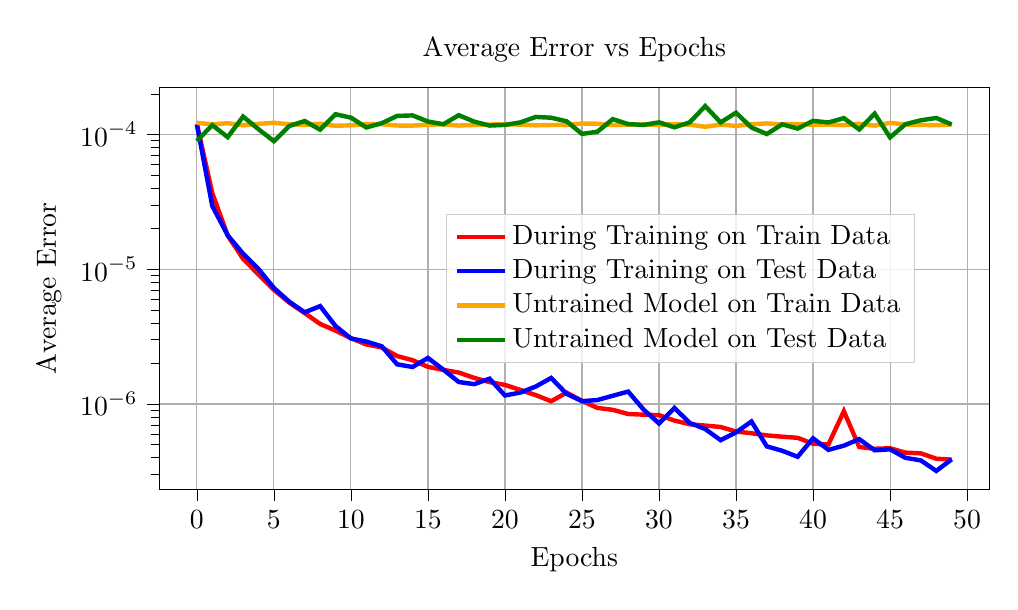
\begin{tikzpicture}

  \definecolor{darkgray176}{RGB}{176,176,176}
  \definecolor{green}{RGB}{0,128,0}
  \definecolor{lightgray204}{RGB}{204,204,204}
  \definecolor{orange}{RGB}{255,165,0}
  
  \begin{axis}[
    width = 1.0\textwidth,
    height = 19em,
  legend cell align={left},
  legend style={
    fill opacity=0.8,
    draw opacity=1,
    text opacity=1,
    at={(0.91,0.5)},
    anchor=east,
    draw=lightgray204
  },
  % log basis y={10},
  tick align=outside,
  tick pos=left,
  title={Average Error vs Epochs},
  x grid style={darkgray176},
  xlabel={Epochs},
  xmajorgrids,
  xmin=-2.45, xmax=51.45,
  xtick style={color=black},
  y grid style={darkgray176},
  ylabel={Average Error},
  ymajorgrids,
  ymin=2.33510655990556e-07, ymax=0.000221454230592227,
  ymode=log,
  ytick style={color=black},
  ytick={1e-08,1e-07,1e-06,1e-05,0.0001,0.001,0.01},
  yticklabels={
    \(\displaystyle {10^{-8}}\),
    \(\displaystyle {10^{-7}}\),
    \(\displaystyle {10^{-6}}\),
    \(\displaystyle {10^{-5}}\),
    \(\displaystyle {10^{-4}}\),
    \(\displaystyle {10^{-3}}\),
    \(\displaystyle {10^{-2}}\)
  }
  ]
  \addplot [ultra thick, red]
table {%
0 0.000119110678497236
1 3.66446620319039e-05
2 1.77629917743616e-05
3 1.19415099106845e-05
4 9.14171869226266e-06
5 7.0352730290324e-06
6 5.64817901249626e-06
7 4.72462261313922e-06
8 3.92743004340446e-06
9 3.50450204678054e-06
10 3.07970799440227e-06
11 2.76725950243417e-06
12 2.6275106392859e-06
13 2.26941324399377e-06
14 2.1133414520591e-06
15 1.88730939498782e-06
16 1.79045071035944e-06
17 1.71247768321336e-06
18 1.56285193497752e-06
19 1.45354010783194e-06
20 1.38544032779464e-06
21 1.27156704365916e-06
22 1.16367743885348e-06
23 1.04827813629527e-06
24 1.21447124001861e-06
25 1.05589560916997e-06
26 9.35082709929702e-07
27 9.04937735413114e-07
28 8.4294913449412e-07
29 8.33415299439366e-07
30 8.2679014212772e-07
31 7.54069617414643e-07
32 7.0767163151686e-07
33 6.91661682594713e-07
34 6.75471369504521e-07
35 6.25178131485882e-07
36 6.06936112035328e-07
37 5.85125235375017e-07
38 5.72119461139664e-07
39 5.61235140139615e-07
40 5.07119239046006e-07
41 5.00920407375816e-07
42 8.84193866568239e-07
43 4.79913239814778e-07
44 4.65450710862569e-07
45 4.69535621050454e-07
46 4.35870873616295e-07
47 4.30478280577518e-07
48 3.92834294871136e-07
49 3.87007872859613e-07
};
\addlegendentry{During Training on Train Data}
\addplot [ultra thick, blue]
table {%
0 0.00011835517216241
1 2.94239616778214e-05
2 1.78588288690662e-05
3 1.30369371618144e-05
4 1.00456127256621e-05
5 7.25863583284081e-06
6 5.73770012124442e-06
7 4.78903893963434e-06
8 5.3246581046551e-06
9 3.79064999833645e-06
10 3.06249035020301e-06
11 2.90575530925707e-06
12 2.68139638137654e-06
13 1.96956534637138e-06
14 1.88275339496613e-06
15 2.19661774281121e-06
16 1.79826713520015e-06
17 1.4568524875358e-06
18 1.40323015784816e-06
19 1.54136819219275e-06
20 1.15701266167889e-06
21 1.21596463031892e-06
22 1.34871140744508e-06
23 1.56057183176017e-06
24 1.1893879445779e-06
25 1.04965113223443e-06
26 1.07065557131136e-06
27 1.15161412850284e-06
28 1.23654535855167e-06
29 9.09538812265964e-07
30 7.17409648132161e-07
31 9.34473348479514e-07
32 7.23355014997651e-07
33 6.52248786536802e-07
34 5.39273003141716e-07
35 6.15782823842892e-07
36 7.42191218705557e-07
37 4.84830366076494e-07
38 4.49736944574397e-07
39 4.06152423693129e-07
40 5.56371048787696e-07
41 4.5693556671722e-07
42 4.90936429287103e-07
43 5.4913465419304e-07
44 4.53623528073877e-07
45 4.61155707398575e-07
46 3.98803734924513e-07
47 3.81665216764304e-07
48 3.18877482641255e-07
49 3.88750692081885e-07
};
\addlegendentry{During Training on Test Data}
\addplot [ultra thick, orange]
table {%
0 0.000121821271022782
1 0.000118786163511686
2 0.000121117249364033
3 0.000116916286060587
4 0.000119748343422543
5 0.000122004646982532
6 0.000118965377623681
7 0.000117821851745248
8 0.000119930613436736
9 0.000115926952275913
10 0.000116842471470591
11 0.000119264717795886
12 0.000119227319373749
13 0.000116418617835734
14 0.000116268653073348
15 0.000118152944196481
16 0.00011861881648656
17 0.000116357769002207
18 0.00011766472744057
19 0.000118461459351238
20 0.000118882810056675
21 0.000118203533929773
22 0.000116807641461492
23 0.000117445903015323
24 0.000117745250463486
25 0.000120490200060885
26 0.000120022261398844
27 0.000117423332994804
28 0.000118374497105833
29 0.000118564435979351
30 0.000118055919301696
31 0.000119002019346226
32 0.00011823955719592
33 0.000113942514872178
34 0.000118257907161023
35 0.00011569067282835
36 0.0001189872782561
37 0.000120693657663651
38 0.000118456307973247
39 0.000119453776278533
40 0.000117906849482097
41 0.000118281546747312
42 0.000117204755952116
43 0.000119701318908483
44 0.000116234936285764
45 0.000121639255667105
46 0.000118501353426836
47 0.000117697200039402
48 0.000117044612125028
49 0.000118546777230222
};
\addlegendentry{Untrained Model on Train Data}
\addplot [ultra thick, green]
table {%
0 8.94988697837107e-05
1 0.000117215560749173
2 9.54625502345152e-05
3 0.000135665308334865
4 0.000109265492937993
5 8.90656738192774e-05
6 0.00011553819058463
7 0.000125691731227562
8 0.000108503714727703
9 0.000141213327879086
10 0.000133093009935692
11 0.000112687819637358
12 0.000121152006613556
13 0.000137145310873166
14 0.000138392802909948
15 0.000124624843010679
16 0.000119010474008974
17 0.000138825504109263
18 0.000124459256767295
19 0.000116323259135243
20 0.000117673094791826
21 0.000122827914310619
22 0.000134805915877223
23 0.000133034307509661
24 0.000125141465105116
25 0.000100915800430812
26 0.000104666156403255
27 0.000129874431877397
28 0.000119255695608445
29 0.000117647301522084
30 0.000122925484902225
31 0.0001129619195126
32 0.000122985773487017
33 0.000162168624228798
34 0.000122765937703662
35 0.000144833509693854
36 0.000112565423478372
37 0.000100688113889191
38 0.000118868752906565
39 0.000110469525679946
40 0.00012610036355909
41 0.000122617464512587
42 0.000132143803057261
43 0.000108827247458976
44 0.000142696153488941
45 9.50354224187322e-05
46 0.000119124881166499
47 0.000127313265693374
48 0.000132477522129193
49 0.000118570867925882
};
\addlegendentry{Untrained Model on Test Data}
\end{axis}

\end{tikzpicture}}\\
  \subfloat[Different Scalars Plus a Single Semi-Positive Definite Matrix$(\tau_k\boldsymbol{S})$]{% This file was created with tikzplotlib v0.10.1.
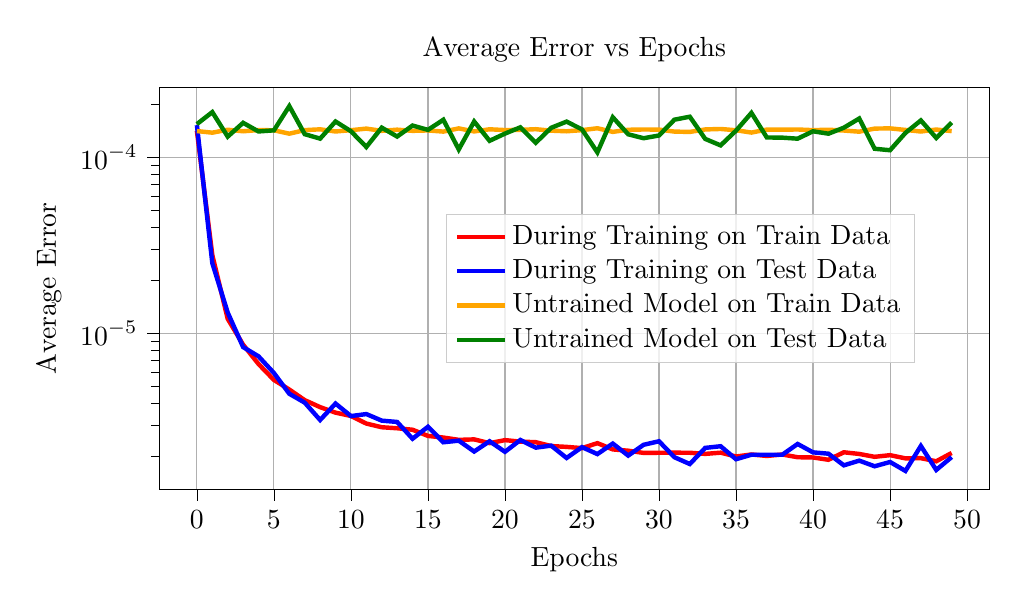
\begin{tikzpicture}

  \definecolor{darkgray176}{RGB}{176,176,176}
  \definecolor{green}{RGB}{0,128,0}
  \definecolor{lightgray204}{RGB}{204,204,204}
  \definecolor{orange}{RGB}{255,165,0}
  
  \begin{axis}[
    width = 1.0\textwidth,
    height = 19em,
  legend cell align={left},
  legend style={
    fill opacity=0.8,
    draw opacity=1,
    text opacity=1,
    at={(0.91,0.5)},
    anchor=east,
    draw=lightgray204
  },
  % log basis y={10},
  tick align=outside,
  tick pos=left,
  title={Average Error vs Epochs},
  x grid style={darkgray176},
  xlabel={Epochs},
  xmajorgrids,
  xmin=-2.45, xmax=51.45,
  xtick style={color=black},
  y grid style={darkgray176},
  ylabel={Average Error},
  ymajorgrids,
  ymin=1.30004957183654e-06, ymax=0.000247303366693065,
  ymode=log,
  ytick style={color=black},
  ytick={1e-07,1e-06,1e-05,0.0001,0.001,0.01},
  yticklabels={
  \(\displaystyle {10^{-7}}\),
  \(\displaystyle {10^{-6}}\),
  \(\displaystyle {10^{-5}}\),
  \(\displaystyle {10^{-4}}\),
  \(\displaystyle {10^{-3}}\),
  \(\displaystyle {10^{-2}}\)
}
  ]
  \addplot [ultra thick, red]
table {%
0 0.000140808770083822
1 2.77877024927875e-05
2 1.20650438475423e-05
3 8.60371164890239e-06
4 6.67991025693482e-06
5 5.42634415978682e-06
6 4.78406172987889e-06
7 4.16472585129668e-06
8 3.80176584258152e-06
9 3.53676637132594e-06
10 3.38710992764391e-06
11 3.06654351334146e-06
12 2.92217282549245e-06
13 2.88355204247637e-06
14 2.82838118437212e-06
15 2.60954288933135e-06
16 2.55327290688001e-06
17 2.47778302764345e-06
18 2.49293429988029e-06
19 2.37284029935836e-06
20 2.46894796873676e-06
21 2.42158648688928e-06
22 2.4035755359364e-06
23 2.28525459533557e-06
24 2.26031443162356e-06
25 2.22407220462628e-06
26 2.37349354392791e-06
27 2.18677610064333e-06
28 2.15019440474862e-06
29 2.08874439522333e-06
30 2.09293762054585e-06
31 2.09529321182345e-06
32 2.09285894925415e-06
33 2.06235563382506e-06
34 2.09541235562938e-06
35 1.99298551706306e-06
36 2.04654361368739e-06
37 2.00757085622172e-06
38 2.0461657186388e-06
39 1.97414806279994e-06
40 1.96775522454118e-06
41 1.90975492841972e-06
42 2.10623920793296e-06
43 2.06045660888776e-06
44 1.98512111637683e-06
45 2.02815704142267e-06
46 1.94528092833934e-06
47 1.95024335880589e-06
48 1.87281955277285e-06
49 2.08697565540206e-06
};
\addlegendentry{During Training on Train Data}
\addplot [ultra thick, blue]
table {%
0 0.000151866624946706
1 2.49946006078972e-05
2 1.30948674268438e-05
3 8.34122874948662e-06
4 7.38843755243579e-06
5 5.93867616771604e-06
6 4.52684344054433e-06
7 4.03162584916572e-06
8 3.21297193295322e-06
9 3.98407746615703e-06
10 3.38162840307632e-06
11 3.47228137798083e-06
12 3.18590946335462e-06
13 3.13101372739766e-06
14 2.51418100560841e-06
15 2.93958305519482e-06
16 2.4015394046728e-06
17 2.45178125624079e-06
18 2.12747499972465e-06
19 2.4323815068783e-06
20 2.11953897633066e-06
21 2.47359025706828e-06
22 2.23747611016734e-06
23 2.29793567996239e-06
24 1.95504912881006e-06
25 2.2525521217176e-06
26 2.05718492907181e-06
27 2.36007554121898e-06
28 2.01702164304152e-06
29 2.32281195167161e-06
30 2.43284330281313e-06
31 1.97447093341907e-06
32 1.80655024450971e-06
33 2.23063898374676e-06
34 2.27990972234693e-06
35 1.92346169569646e-06
36 2.03991839953233e-06
37 2.03988429348101e-06
38 2.03888680516684e-06
39 2.34781578001275e-06
40 2.10382722798386e-06
41 2.0672875962191e-06
42 1.77587082816899e-06
43 1.88824776614638e-06
44 1.75387231138302e-06
45 1.85520821105456e-06
46 1.65030076004768e-06
47 2.28701583182556e-06
48 1.67188488831016e-06
49 1.97793519873812e-06
};
\addlegendentry{During Training on Test Data}
\addplot [ultra thick, orange]
table {%
0 0.00014060313696973
1 0.000137656141305342
2 0.000143065073643811
3 0.000140192554681562
4 0.000142427845275961
5 0.000142034099553712
6 0.000135852737003006
7 0.00014235639537219
8 0.000143847602885216
9 0.00013983370445203
10 0.000142199758556671
11 0.000145203914144076
12 0.00014099404506851
13 0.000143194061820395
14 0.000140986638143659
15 0.000141734140925109
16 0.000139620620757341
17 0.000145604368299246
18 0.000139923329697922
19 0.000143899538670667
20 0.000142461081850342
21 0.000142865843372419
22 0.000144075427670032
23 0.000141339376568794
24 0.000140182426548563
25 0.000142293807584792
26 0.000145876678288914
27 0.000139112686156295
28 0.000143021941767074
29 0.000143526252941228
30 0.000143316239700653
31 0.000139636162202805
32 0.000139017691253684
33 0.000143602766911499
34 0.000144505393109284
35 0.000142094271723181
36 0.000137869006721303
37 0.000143355937325396
38 0.000143186174682342
39 0.000143536293762736
40 0.000142327175126411
41 0.000143050288897939
42 0.00014157967234496
43 0.000139441690407693
44 0.000145230937050655
45 0.000145648096804507
46 0.000142689401400276
47 0.000139756724820472
48 0.000143463927088305
49 0.00014049097080715
};
\addlegendentry{Untrained Model on Train Data}
\addplot [ultra thick, green]
table {%
0 0.000154029330587946
1 0.000180180853931233
2 0.000130726533825509
3 0.000156632129801437
4 0.000139883763040416
5 0.000141912765684538
6 0.000194816995644942
7 0.000135004651383497
8 0.000127355684526265
9 0.000159308925503865
10 0.000140322328661568
11 0.000114190057502128
12 0.000147035854752176
13 0.00013088078412693
14 0.000151125670527108
15 0.000142780350870453
16 0.000163049713592045
17 0.000110557492007501
18 0.00015931720554363
19 0.000123746853205375
20 0.00013601804676
21 0.000147675746120512
22 0.000120715449156705
23 0.000146728663821705
24 0.000159101778990589
25 0.000143717334140092
26 0.00010641503467923
27 0.000168388287420385
28 0.000134773305035196
29 0.000128033978398889
30 0.000132704633870162
31 0.00016315164975822
32 0.000169641323736869
33 0.000126891216496006
34 0.000116580682515632
35 0.000141325872391462
36 0.000178295289515518
37 0.000129308318719268
38 0.00012899779540021
39 0.000127264560433105
40 0.000140162432217039
41 0.000135849215439521
42 0.000146909078466706
43 0.000165729303262196
44 0.00011155797255924
45 0.000109411274024751
46 0.000137256662128493
47 0.00016158472863026
48 0.000128560437588021
49 0.000157007976667956
};
\addlegendentry{Untrained Model on Test Data}
\end{axis}

\end{tikzpicture}}\\
  \caption{Training the \ac{URWF} Algorithm in different Scenarios Without Optuna\cite{Akiba2019}}
  \label{fig:urwf_training_04_05_06}
  \end{figure}
%   \clearpage % End the page
}
\afterpage{%
%   \clearpage % Start a new page
\begin{figure}[!htbp]
  \subfloat[Different Matrices$(\boldsymbol{M}_k)$]{% This file was created with tikzplotlib v0.10.1.
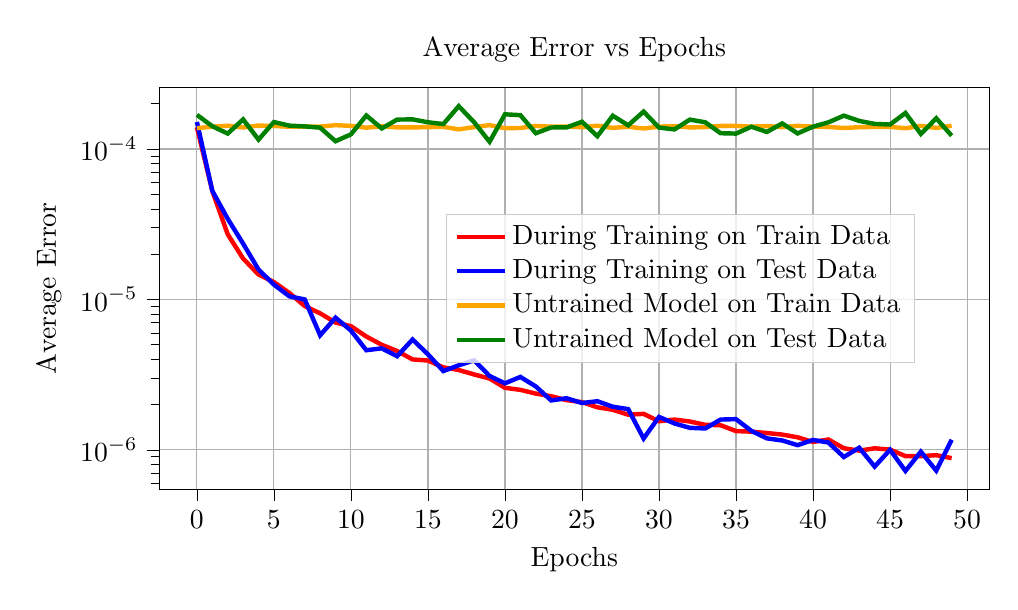
\begin{tikzpicture}

  \definecolor{darkgray176}{RGB}{176,176,176}
  \definecolor{green}{RGB}{0,128,0}
  \definecolor{lightgray204}{RGB}{204,204,204}
  \definecolor{orange}{RGB}{255,165,0}
  
  \begin{axis}[
    width = 1.0\textwidth,
    height = 19em,
  legend cell align={left},
  legend style={
    fill opacity=0.8,
    draw opacity=1,
    text opacity=1,
    at={(0.91,0.5)},
    anchor=east,
    draw=lightgray204
  },
  % log basis y={10},
  tick align=outside,
  tick pos=left,
  title={Average Error vs Epochs},
  x grid style={darkgray176},
  xlabel={Epochs},
  xmajorgrids,
  xmin=-2.45, xmax=51.45,
  xtick style={color=black},
  y grid style={darkgray176},
  ylabel={Average Error},
  ymajorgrids,
  ymin=5.47956319196448e-07, ymax=0.000254691381547786,
  ymode=log,
  ytick style={color=black},
  ytick={1e-08,1e-07,1e-06,1e-05,0.0001,0.001,0.01},
  yticklabels={
    \(\displaystyle {10^{-8}}\),
    \(\displaystyle {10^{-7}}\),
    \(\displaystyle {10^{-6}}\),
    \(\displaystyle {10^{-5}}\),
    \(\displaystyle {10^{-4}}\),
    \(\displaystyle {10^{-3}}\),
    \(\displaystyle {10^{-2}}\)
  }
  ]
  \addplot [ultra thick, red]
table {%
0 0.000139422554639168
1 5.25441355421208e-05
2 2.709246109589e-05
3 1.86883116839454e-05
4 1.4641495909018e-05
5 1.30382604766055e-05
6 1.10479877548642e-05
7 9.03117143025156e-06
8 8.08377171779284e-06
9 7.014934453764e-06
10 6.64117942505982e-06
11 5.66791140954592e-06
12 4.99323004987673e-06
13 4.53997472504852e-06
14 3.99270811612951e-06
15 3.92411902794265e-06
16 3.53491191162902e-06
17 3.39455823450407e-06
18 3.1713191219751e-06
19 2.97965834761271e-06
20 2.58465047409118e-06
21 2.5051617740246e-06
22 2.36605910686194e-06
23 2.27213763537293e-06
24 2.14105693885358e-06
25 2.07581410904822e-06
26 1.91861840903584e-06
27 1.84637030997692e-06
28 1.71315411989781e-06
29 1.73497676314582e-06
30 1.54966937770951e-06
31 1.59103592523024e-06
32 1.54397719143162e-06
33 1.46790443977807e-06
34 1.45789761063497e-06
35 1.33272737912193e-06
36 1.32122954710212e-06
37 1.2942375633429e-06
38 1.26361408092635e-06
39 1.21193875202152e-06
40 1.12860448098218e-06
41 1.17169065561029e-06
42 1.0251166031594e-06
43 9.8811494808615e-07
44 1.02411047464557e-06
45 1.00423574167507e-06
46 9.08802235244366e-07
47 9.08564288693015e-07
48 9.21839614420605e-07
49 8.81109031070082e-07
};
\addlegendentry{During Training on Train Data}
\addplot [ultra thick, blue]
table {%
0 0.000151191532495432
1 5.27330812474247e-05
2 3.43467727361713e-05
3 2.34825092775282e-05
4 1.57967224367894e-05
5 1.25444585137302e-05
6 1.04895107142511e-05
7 9.99405347101856e-06
8 5.77313267058344e-06
9 7.56428335080273e-06
10 6.20858509137179e-06
11 4.59601551483502e-06
12 4.72754800284747e-06
13 4.19237494497793e-06
14 5.41578947377275e-06
15 4.31831585956388e-06
16 3.34092874254566e-06
17 3.64814991371532e-06
18 3.93835989598301e-06
19 3.09812821797095e-06
20 2.76999890047591e-06
21 3.05379262499628e-06
22 2.63992797044921e-06
23 2.13079511013348e-06
24 2.2038937004254e-06
25 2.0483175831032e-06
26 2.10558482649503e-06
27 1.93491723621264e-06
28 1.86590375506057e-06
29 1.18982120511646e-06
30 1.65560504683526e-06
31 1.49886989220249e-06
32 1.40136648951739e-06
33 1.38726443310588e-06
34 1.5903664234429e-06
35 1.600476934982e-06
36 1.33635251131636e-06
37 1.19272579013341e-06
38 1.15448892756831e-06
39 1.07466962617764e-06
40 1.16404714844975e-06
41 1.11877704966901e-06
42 8.96443566489324e-07
43 1.03346019386663e-06
44 7.74358625221794e-07
45 1.00108979950164e-06
46 7.24411620467436e-07
47 9.72342604654841e-07
48 7.2755648261591e-07
49 1.16638921099366e-06
};
\addlegendentry{During Training on Test Data}
\addplot [ultra thick, orange]
table {%
0 0.000137548107886687
1 0.000140638832817785
2 0.000142808101372793
3 0.000138855073601007
4 0.00014315867156256
5 0.000142147371661849
6 0.000140535441460088
7 0.000140832271426916
8 0.000141012889798731
9 0.000143917815876193
10 0.000142426055390388
11 0.000138538351166062
12 0.000141437121783383
13 0.000139053459861316
14 0.000139040130306967
15 0.000139728872454725
16 0.000140273332362995
17 0.00013496758765541
18 0.000139760843012482
19 0.000144059871672653
20 0.000137425566208549
21 0.000137912458740175
22 0.000142265387694351
23 0.000140677715535276
24 0.000141052427352406
25 0.000139516676426865
26 0.00014278301387094
27 0.000138091811095364
28 0.000140507239848375
29 0.000136786737130024
30 0.00014075510262046
31 0.000142040196806192
32 0.000139078518259339
33 0.000139772397233173
34 0.000142270961077884
35 0.000142297969432548
36 0.000140746793476865
37 0.000141959739266895
38 0.000139722877065651
39 0.000142463482916355
40 0.000140872885822318
41 0.00014001976524014
42 0.000137886876473203
43 0.000139517200295813
44 0.00014015486522112
45 0.000140228410600685
46 0.000137308554258198
47 0.00014238734729588
48 0.000138002840685658
49 0.000142704491736367
};
\addlegendentry{Untrained Model on Train Data}
\addplot [ultra thick, green]
table {%
0 0.000168594866408966
1 0.000141678872751072
2 0.000126560087664984
3 0.000157214250066318
4 0.000115438073407859
5 0.000150999199831858
6 0.000142947799758986
7 0.000141304670250975
8 0.000138527931994759
9 0.000112627378257457
10 0.000125072823720984
11 0.000166890022228472
12 0.000136944450787269
13 0.000156815774971619
14 0.000157319751451723
15 0.000150483218021691
16 0.000146467093145475
17 0.00019265255832579
18 0.000150442734593526
19 0.000111669789475854
20 0.000169916238519363
21 0.000167860955116339
22 0.000127240127767436
23 0.000138955030706711
24 0.000139115072670393
25 0.000151672968058847
26 0.000121595592645463
27 0.000166218713275157
28 0.000143689205287956
29 0.000177146794158034
30 0.000138729737955146
31 0.000134799440274946
32 0.00015673965390306
33 0.000150496722199023
34 0.000127258579595946
35 0.000126562154036947
36 0.000140600168379024
37 0.000129729727632366
38 0.000147858329000883
39 0.000126872822875157
40 0.000140709613333456
41 0.000150389416376129
42 0.000166537720360793
43 0.000153616216266528
44 0.000146757418406196
45 0.000145377474837005
46 0.000173495995113626
47 0.000125866179587319
48 0.000159938761498779
49 0.000122543351608329
};
\addlegendentry{Untrained Model on Test Data}
\end{axis}

\end{tikzpicture}}\\  
  \subfloat[Different Semi-Positive Definite Matrices$(\boldsymbol{S}_k)$]{% This file was created with tikzplotlib v0.10.1.
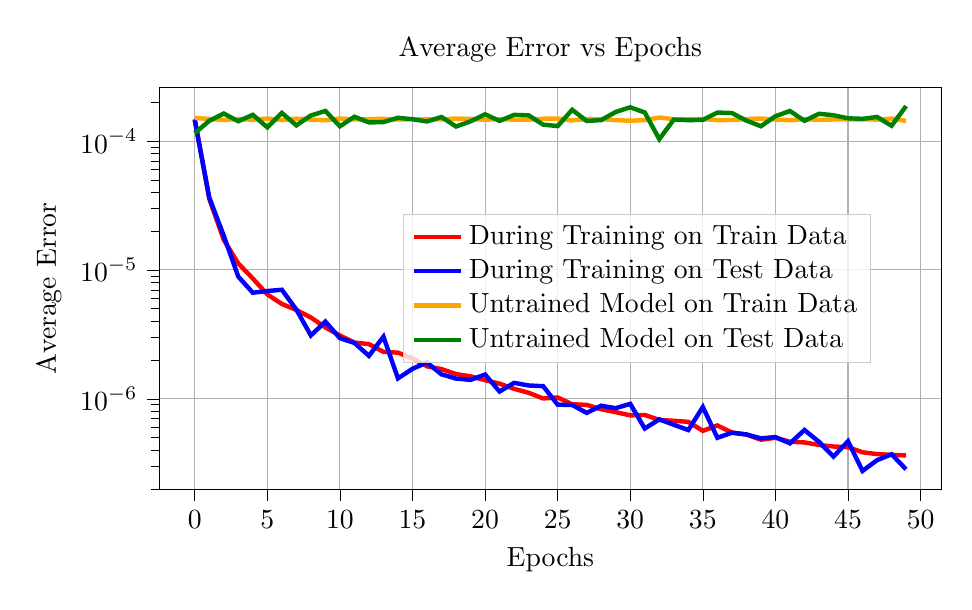
\begin{tikzpicture}

  \definecolor{darkgray176}{RGB}{176,176,176}
  \definecolor{green}{RGB}{0,128,0}
  \definecolor{lightgray204}{RGB}{204,204,204}
  \definecolor{orange}{RGB}{255,165,0}
  
  \begin{axis}[
    width = 0.95\textwidth,
    height = 19em,
  legend cell align={left},
  legend style={
    fill opacity=0.8,
    draw opacity=1,
    text opacity=1,
    at={(0.91,0.5)},
    anchor=east,
    draw=lightgray204
  },
  % log basis y={10},
  tick align=outside,
  tick pos=left,
  title={Average Error vs Epochs},
  x grid style={darkgray176},
  xlabel={Epochs},
  xmajorgrids,
  xmin=-2.45, xmax=51.45,
  xtick style={color=black},
  y grid style={darkgray176},
  ylabel={Average Error},
  ymajorgrids,
  ymin=1.98989848731464e-07, ymax=0.00025862395496495,
  ymode=log,
  ytick style={color=black},
  ytick={1e-08,1e-07,1e-06,1e-05,0.0001,0.001,0.01},
  yticklabels={
    \(\displaystyle {10^{-8}}\),
    \(\displaystyle {10^{-7}}\),
    \(\displaystyle {10^{-6}}\),
    \(\displaystyle {10^{-5}}\),
    \(\displaystyle {10^{-4}}\),
    \(\displaystyle {10^{-3}}\),
    \(\displaystyle {10^{-2}}\)
  }
  ]
  \addplot [ultra thick, red]
  table {%
  0 0.000148013044963591
  1 3.56593227479607e-05
  2 1.7092230336857e-05
  3 1.12235911728931e-05
  4 8.58035764395026e-06
  5 6.45710269964184e-06
  6 5.44462363905041e-06
  7 4.88857358504902e-06
  8 4.2726201172627e-06
  9 3.58169586434087e-06
  10 3.09524739350309e-06
  11 2.73389900939947e-06
  12 2.65521657638601e-06
  13 2.31281637752545e-06
  14 2.27968439503456e-06
  15 2.05286619348044e-06
  16 1.78653704097087e-06
  17 1.69934662608284e-06
  18 1.55517341227096e-06
  19 1.49384698033828e-06
  20 1.3938711163064e-06
  21 1.30992964386678e-06
  22 1.19467654258187e-06
  23 1.11279143766296e-06
  24 1.00586737517006e-06
  25 1.02330841400544e-06
  26 9.0733004753929e-07
  27 8.96316521448171e-07
  28 8.29465079732472e-07
  29 7.87274132107996e-07
  30 7.43528971725027e-07
  31 7.48820809803874e-07
  32 6.85715860981873e-07
  33 6.74960119795287e-07
  34 6.62006982565799e-07
  35 5.64021263471659e-07
  36 6.21000424416707e-07
  37 5.4747005151512e-07
  38 5.2761015467695e-07
  39 4.81172207855707e-07
  40 4.98232964218914e-07
  41 4.6397821051869e-07
  42 4.58541705938842e-07
  43 4.38037005778824e-07
  44 4.26196010039348e-07
  45 4.2150298895649e-07
  46 3.84383071150296e-07
  47 3.72081899513432e-07
  48 3.67385837307665e-07
  49 3.63334208941524e-07
  };
  \addlegendentry{During Training on Train Data}
  \addplot [ultra thick, blue]
  table {%
  0 0.000145961690577678
  1 3.6507273762254e-05
  2 1.83924421435222e-05
  3 8.87434453034075e-06
  4 6.65402694721706e-06
  5 6.85723716742359e-06
  6 7.01677663528244e-06
  7 4.92142953589791e-06
  8 3.10200198327948e-06
  9 3.96965651816572e-06
  10 2.95227073365822e-06
  11 2.71325984613213e-06
  12 2.15284285332018e-06
  13 3.03261163026036e-06
  14 1.43896522786235e-06
  15 1.70873647675762e-06
  16 1.90969149116427e-06
  17 1.54746635416814e-06
  18 1.43470697366865e-06
  19 1.4017372222952e-06
  20 1.54278404806973e-06
  21 1.13814337510121e-06
  22 1.32910520278529e-06
  23 1.26849226944614e-06
  24 1.25276187645795e-06
  25 9.00273789739003e-07
  26 8.95020548341563e-07
  27 7.7743254678353e-07
  28 8.83171367149771e-07
  29 8.45460078835458e-07
  30 9.13137625957461e-07
  31 5.87568308674236e-07
  32 6.92485286890587e-07
  33 6.28680254521896e-07
  34 5.71698194562487e-07
  35 8.63643435877748e-07
  36 4.98133147175395e-07
  37 5.44820807135693e-07
  38 5.29007309069129e-07
  39 4.93094887588086e-07
  40 5.04310378346418e-07
  41 4.50991336720108e-07
  42 5.72123838082916e-07
  43 4.63405569917086e-07
  44 3.56029943304748e-07
  45 4.6835725697747e-07
  46 2.75656987014372e-07
  47 3.33770287852531e-07
  48 3.71070939308993e-07
  49 2.83416682123061e-07
  };
  \addlegendentry{During Training on Test Data}
  \addplot [ultra thick, orange]
  table {%
  0 0.000151286862092093
  1 0.000148271938087419
  2 0.000145962316310033
  3 0.000148140708915889
  4 0.000146270336699672
  5 0.000149768020492047
  6 0.000145538549986668
  7 0.000149274768773466
  8 0.000146568301715888
  9 0.000144949066452682
  10 0.00014968030154705
  11 0.000146915088407695
  12 0.000148198654642329
  13 0.000148643390275538
  14 0.000147157494211569
  15 0.000147706436109729
  16 0.00014777151227463
  17 0.00014694788842462
  18 0.000149669518577866
  19 0.000148425155202858
  20 0.000146184596815147
  21 0.000148376799188554
  22 0.000146324280649424
  23 0.00014655634004157
  24 0.000149089726619422
  25 0.000149657396832481
  26 0.000144709527376108
  27 0.000148061357322149
  28 0.000147991930134594
  29 0.000145307276397943
  30 0.000143848243169487
  31 0.000145373909617774
  32 0.000152415770571679
  33 0.000147752347402275
  34 0.00014776736497879
  35 0.000147837854456156
  36 0.000145569443702698
  37 0.000145633559441194
  38 0.000148161940160207
  39 0.000149608822539449
  40 0.000146714635775425
  41 0.000145101090311073
  42 0.000147954560816288
  43 0.000146047284943052
  44 0.000147063998156227
  45 0.000147197628393769
  46 0.000147608181578107
  47 0.000146761129144579
  48 0.000149398503708653
  49 0.000143366807606071
  };
  \addlegendentry{Untrained Model on Train Data}
  \addplot [ultra thick, green]
  table {%
  0 0.000115061491669621
  1 0.000143547338666394
  2 0.000163512173458003
  3 0.000142517077620141
  4 0.000159814182552509
  5 0.00012783041165676
  6 0.000165362667758018
  7 0.000132426110212691
  8 0.000157876085722819
  9 0.000171300649526529
  10 0.000130172455101274
  11 0.000154473222210072
  12 0.000139474926982075
  13 0.000140412186738104
  14 0.000151597065269016
  15 0.00014767273387406
  16 0.000141933254781179
  17 0.000153813511133194
  18 0.000129606123664416
  19 0.000142261982546188
  20 0.000161294257850386
  21 0.00014334442676045
  22 0.000159681003424339
  23 0.000158348615514114
  24 0.000134108049678616
  25 0.000130705229821615
  26 0.000174892600625753
  27 0.000143100725836121
  28 0.000145519719808362
  29 0.000168184196809307
  30 0.000182958712684922
  31 0.000166574260219932
  32 0.000103557540569454
  33 0.000146681413752958
  34 0.000145311874803156
  35 0.00014605671458412
  36 0.000166460915352218
  37 0.000165033299708739
  38 0.000144075253047049
  39 0.000130360465846024
  40 0.000155840680235997
  41 0.000171156978467479
  42 0.000143605619086884
  43 0.000162815587827936
  44 0.000158585360622965
  45 0.000150236810441129
  46 0.000148762876051478
  47 0.000153807501192205
  48 0.000131454333313741
  49 0.000186694131116383
  };
  \addlegendentry{Untrained Model on Test Data}
  \end{axis}
  
  \end{tikzpicture}
  }\\  
  \subfloat[Proposed Scenario Using Optuna\cite{Akiba2019}: Different Scalars Plus a Single Semi-Positive Definite Matrix$(\tau_k\boldsymbol{S})$, $lr=7.622\times10^{-3}$]{% This file was created with tikzplotlib v0.10.1.
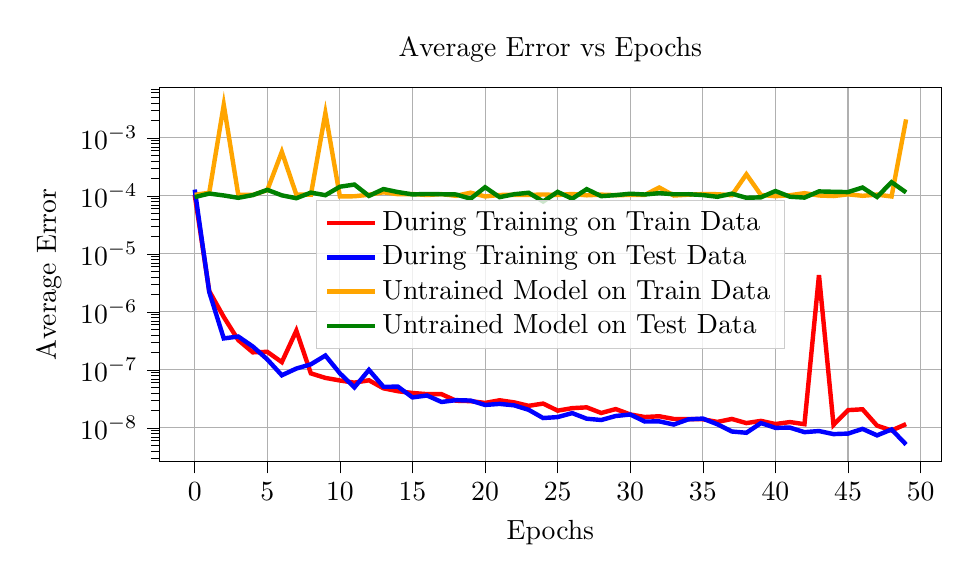
\begin{tikzpicture}

    \definecolor{darkgray176}{RGB}{176,176,176}
    \definecolor{green}{RGB}{0,128,0}
    \definecolor{lightgray204}{RGB}{204,204,204}
    \definecolor{orange}{RGB}{255,165,0}
    
    \begin{axis}[
      width = 0.95\textwidth,
      height = 18em,
    legend cell align={left},
    legend style={
      fill opacity=0.8,
      draw opacity=1,
      text opacity=1,
      at={(0.5,0.5)},
      anchor=center,
      draw=lightgray204
    },
    % log basis y={10},
    tick align=outside,
    tick pos=left,
    title={Average Error vs Epochs},
    x grid style={darkgray176},
    xlabel={Epochs},
    xmajorgrids,
    xmin=-2.45, xmax=51.45,
    xtick style={color=black},
    y grid style={darkgray176},
    ylabel={Average Error},
    ymajorgrids,
    ymin=2.63604330184737e-09, ymax=0.00725950156863836,
    ymode=log,
    ytick style={color=black},
    ytick={1e-10,1e-09,1e-08,1e-07,1e-06,1e-05,0.0001,0.001,0.01,0.1},
    yticklabels={
      \(\displaystyle {10^{-10}}\),
      \(\displaystyle {10^{-9}}\),
      \(\displaystyle {10^{-8}}\),
      \(\displaystyle {10^{-7}}\),
      \(\displaystyle {10^{-6}}\),
      \(\displaystyle {10^{-5}}\),
      \(\displaystyle {10^{-4}}\),
      \(\displaystyle {10^{-3}}\),
      \(\displaystyle {10^{-2}}\),
      \(\displaystyle {10^{-1}}\)
    }
    ]
    \addplot [ultra thick, red]
    table {%
    0 0.000104205340903718
    1 2.2795081804361e-06
    2 8.16013880466926e-07
    3 3.26127519656438e-07
    4 2.00797316551871e-07
    5 2.04524624791702e-07
    6 1.36023288632714e-07
    7 4.74071129019649e-07
    8 8.70571454925084e-08
    9 7.27430773395099e-08
    10 6.5652713487907e-08
    11 6.02018914719338e-08
    12 6.61969394855078e-08
    13 4.81310458155804e-08
    14 4.2873633532281e-08
    15 3.99703772302473e-08
    16 3.81714855279824e-08
    17 3.8142367486671e-08
    18 2.93974711240708e-08
    19 2.89232531258676e-08
    20 2.69239741612637e-08
    21 2.99225142441628e-08
    22 2.75352860512612e-08
    23 2.4009436216943e-08
    24 2.62635957426482e-08
    25 1.98318286237509e-08
    26 2.18844142807484e-08
    27 2.25979448487124e-08
    28 1.80841581709501e-08
    29 2.10961470514803e-08
    30 1.70547433953061e-08
    31 1.53920822754117e-08
    32 1.58656572324389e-08
    33 1.42510874212576e-08
    34 1.41820661880843e-08
    35 1.4081289023693e-08
    36 1.26731078964326e-08
    37 1.42557086135753e-08
    38 1.21001750841288e-08
    39 1.32015909315442e-08
    40 1.16595693100408e-08
    41 1.26017134505219e-08
    42 1.15926468424732e-08
    43 4.30966929343413e-06
    44 1.12703659738145e-08
    45 2.02334238252888e-08
    46 2.09316262100856e-08
    47 1.09466631315058e-08
    48 9.01701913136321e-09
    49 1.16273870531813e-08
    };
    \addlegendentry{During Training on Train Data}
    \addplot [ultra thick, blue]
    table {%
    0 0.000128205894725397
    1 2.19211028706923e-06
    2 3.48693362184349e-07
    3 3.7564521448985e-07
    4 2.53075398859437e-07
    5 1.51381684077023e-07
    6 8.07240780886787e-08
    7 1.05399159622266e-07
    8 1.24686110325456e-07
    9 1.76708667254388e-07
    10 8.71838210514397e-08
    11 4.9951530911585e-08
    12 9.98501263893559e-08
    13 5.1198544070985e-08
    14 5.13218765263446e-08
    15 3.35316165944732e-08
    16 3.61962158024198e-08
    17 2.79910761236124e-08
    18 3.00771283434642e-08
    19 2.95923321402825e-08
    20 2.4853880731257e-08
    21 2.59286903059319e-08
    22 2.44853541886414e-08
    23 2.05111181372786e-08
    24 1.47937218031302e-08
    25 1.5353929683215e-08
    26 1.79923898002698e-08
    27 1.44036702565131e-08
    28 1.36676279183234e-08
    29 1.603949861817e-08
    30 1.70154574874459e-08
    31 1.28716752811897e-08
    32 1.29476260823935e-08
    33 1.14277387552875e-08
    34 1.4037178530657e-08
    35 1.44796095113975e-08
    36 1.15444818149513e-08
    37 8.66101146357323e-09
    38 8.24099988250282e-09
    39 1.21144925202543e-08
    40 1.00226200672182e-08
    41 1.01044204114942e-08
    42 8.44652703335669e-09
    43 8.82723494299853e-09
    44 7.81588394005439e-09
    45 7.98052735007104e-09
    46 9.61182422543061e-09
    47 7.4352684009682e-09
    48 9.4029859454281e-09
    49 5.17222886742275e-09
    };
    \addlegendentry{During Training on Test Data}
    \addplot [ultra thick, orange]
    table {%
    0 0.000104004502645694
    1 0.000113090267404914
    2 0.00369982863776386
    3 0.000103595812106505
    4 0.000103680438769516
    5 0.000125327438581735
    6 0.000573276192881167
    7 0.000104799939435907
    8 0.000104467922938056
    9 0.00266967760398984
    10 9.74361173575744e-05
    11 9.83515856205486e-05
    12 0.000104475227999501
    13 0.000115149639896117
    14 0.000106749808765016
    15 0.000107450287032407
    16 0.000103390899312217
    17 0.000107067287899554
    18 0.000100105462479405
    19 0.000113200912892353
    20 9.77006420725957e-05
    21 0.000103448765003122
    22 0.000104000508144964
    23 0.000103353981103282
    24 0.000105591047031339
    25 0.000103221151221078
    26 0.00010765408660518
    27 0.000102091478765942
    28 0.000104882899904624
    29 0.000102825011708774
    30 0.000103528509498574
    31 0.000103895661595743
    32 0.000138981064083055
    33 0.000101232988527045
    34 0.000104792459751479
    35 0.000107034466054756
    36 0.000106611536466517
    37 0.000102448932011612
    38 0.000235152678214945
    39 0.000103626218333375
    40 9.85821752692573e-05
    41 0.000102437457826454
    42 0.000111155663034879
    43 0.000101380828709807
    44 9.91987908491865e-05
    45 0.000106175990367774
    46 0.000100137636763975
    47 0.000104896309494507
    48 9.75669390754774e-05
    49 0.00207684771157801
    };
    \addlegendentry{Untrained Model on Train Data}
    \addplot [ultra thick, green]
    table {%
    0 9.51192560023628e-05
    1 0.000109474291093647
    2 0.000101536650618073
    3 9.24414925975725e-05
    4 0.000102999874798115
    5 0.000126819082652219
    6 0.000101982383057475
    7 9.10065864445642e-05
    8 0.000113746289571282
    9 0.000102590936876368
    10 0.000143659664900042
    11 0.000156529058585875
    12 9.96770613710396e-05
    13 0.000130805958178826
    14 0.000116074705147184
    15 0.000105866813100874
    16 0.000107682615634985
    17 0.000106509614852257
    18 0.000105575592897367
    19 8.92794705578126e-05
    20 0.000140646734507754
    21 9.49161913013086e-05
    22 0.000106560277345125
    23 0.000113010035420302
    24 7.99219124019146e-05
    25 0.00011702597112162
    26 8.920714026317e-05
    27 0.000130467757117003
    28 9.88191241049208e-05
    29 0.000102830796095077
    30 0.000108744738099631
    31 0.000105451188574079
    32 0.000111337336420547
    33 0.000106409403088037
    34 0.000106660001620185
    35 0.000103220765595324
    36 9.62638878263533e-05
    37 0.000108933658339083
    38 9.25103668123484e-05
    39 9.42573096835986e-05
    40 0.000121093005873263
    41 9.66605221037753e-05
    42 9.32564653339796e-05
    43 0.000119190364785027
    44 0.000117450043035205
    45 0.0001160800238722
    46 0.000139031486469321
    47 9.57154188654386e-05
    48 0.000171932319062762
    49 0.000114621827378869
    };
    \addlegendentry{Untrained Model on Test Data}
    \end{axis}
    
    \end{tikzpicture}
    }\\  
  \caption{Training the \ac{URWF} Algorithm in different Scenarios With and Without Optuna\cite{Akiba2019}}
  \label{fig:urwf_training_07_08_optuna}
  \end{figure}
%   \clearpage % End the page
}




\section*{Ideas for Future Work}

I can think of a couple of directions to go on from here and I would like to express them.

\subsection*{Different Variants/Different Applications}

There are many \ac{WF} variants out there and we can expect more to appear in the future. Currently \cite{Liu2019}\cite{Jaganathan2015} 
give an overview of \ac{WF} variants and you might want to start from there for \ac{DU}/\ac{AU} on those variants. I for one would 
love to see the result of fine tuning a \ac{DU}/\ac{AU} version of a \ac{WF} variant for a specific real world problem like\cite{Fogel2013}. 

\subsection*{Data}

Having parsimonious data representation\cite{Foucart2013} and data with noise are worth looking into.

\subsection*{Different Scenarios}

Depending on the function we are trying to minimize and the iterative \ac{WF} variant algorithm we are unfolding/unrolling 
it is possible to investigate other scenarios for parameter learning too. Possible candidate are but not limited to:

\begin{itemize}
  \item conjugate operator $\boldsymbol{A}^*$,
  % \item weights of the measurements $c_j$,
  \item Giving weights to the sampling operation by $\left|\phi(\boldsymbol{A}_j\psi)-G_j\right|_X^2 \rightarrow \left|c_j \odot \left(\phi(\boldsymbol{A}_j\psi)-G_j\right)\right|_X^2$ and optimizing the $c_j$s.
  \item Regularizer's weight $\lambda$.
\end{itemize}









